\documentclass[sigconf]{acmart}

\fancyhf{} % Remove fancy page headers 
% \fancyhead[C]{Anonymous submission \#9999 to ACM CCS 2017} % TODO: replace 9999 with your paper number
\fancyfoot[C]{\thepage}

\setcopyright{none} % No copyright notice required for submissions
% \acmConference[Anonymous Submission to ACM CCS 2017]{ACM Conference on Computer and Communications Security}{Due 19 May 2017}{Dallas, Texas}
% \acmYear{2017}

\settopmatter{printacmref=false, printccs=true, printfolios=true} % We want page numbers on submissions

%%\ccsPaper{9999} % TODO: replace with your paper number once obtained

%packages
\usepackage{natbib}
\usepackage{amsmath}
\usepackage{amsthm}
\usepackage{mathtools}
\usepackage{mdframed}
\usepackage{subfigure}
\usepackage{booktabs}
% \usepackage{hyperref}
\usepackage{subfigure}
\usepackage{siunitx} % Provides the \SI{}{} and \si{} command for typesetting SI units
\usepackage{graphicx} % Required for the inclusion of images
% \usepackage{natbib} % Required to change bibliography style to APA
\usepackage{datetime}
\usepackage{lscape}
\usepackage{algorithm}
\usepackage{algorithmic}
\usepackage{xspace}
\usepackage[english]{babel} % English language/hyphenation
\usepackage{proof}
\usepackage{booktabs} % Top and bottom rules for tables
\usepackage[colorlinks, allcolors = blue,]{hyperref}
\usepackage{accents}
\usepackage{amsfonts}
\usepackage{stmaryrd}
\usepackage{amsmath,amsthm,amssymb,latexsym} 
\usepackage{microtype}
\usepackage{graphicx}
\usepackage{subfigure}
\usepackage{booktabs} % for professional tables
\usepackage{hyperref}
\usepackage{icml2019}
\usepackage{lipsum}

\usepackage{authblk}


%new commands
\newcommand{\theHalgorithm}{\arabic{algorithm}}
\newtheorem{definition}{Definition}
\usepackage{cancel}
\usepackage[normalem]{ulem}
\newcommand{\dataobs}{\textbf{x}}
\newcommand{\adj}[2]{\textbf{adj}(#1,#2)}
\newcommand{\candidateset}{\mathcal{R}_{\textup{post}}}
\newcommand{\bprior}{\boldsymbol{\beta}_{\textup{prior}}}
\newcommand{\bysinfer}{\mathsf{Infer}}
\newcommand{\betad}{\mathsf{Beta}}
\newcommand{\betaf}{\textup{B}}
\newcommand{\mbetaf}{\boldsymbol{\textup{B}}}
\newcommand{\vtheta}{\boldsymbol{\theta}}
\newcommand{\valpha}{\boldsymbol{\alpha}}
\newcommand{\vbeta}{\boldsymbol{\beta}}
\newcommand{\lapmech}{\mathsf{LSDim}}
\newcommand{\ilapmech}{\mathsf{LSHist}}
\newcommand{\binomial}[2]{\mathsf{Bin}(#1, #2)}
\newcommand{\multinomial}[2]{\mathsf{Mult}(#1, #2)}
\newcommand{\expmech}{\mathsf{EHD}}
\newcommand{\hexpmech}{\mathsf{EHDS}}
\newcommand{\lexpmech}{\mathsf{EHDL}}
\newcommand{\hexpmechd}{\mathsf{expMech}^{D}_{\hellinger}}
\newcommand{\privinfer}{\mathsf{PrivInfer}}
\newcommand{\hlg}{\mathsf{H}}
\newcommand{\dirichlet}[1]{\mathsf{Dir}(#1)}
\newcommand{\alphas}{\boldsymbol{\alpha}}
\newcommand{\xis}{\boldsymbol{\xi}}
\newcommand{\iverson}[1]{[#1]}
\newcommand{\datauni}{\mathcal{X}}
\newcommand{\hellinger}{\mathcal{H}}
\newcommand{\ux}[1]{u(\textbf{x}, {#1})}
\newcommand{\uxadj}[1]{u(\textbf{x}', {#1})}
\newcommand{\cardinality}[2]{\mathcal{C}^{#1}_{#2}}
\newcommand{\range}{\mathcal{O}}
\newcommand{\nomalizer}[1]{\sum\limits_{r'\in \mathcal{R}_{\textup{post}}} \exp \big(\frac{-\epsilon\cdot \mathcal{H} (\mathsf{BI}(#1),r')}{4 \cdot S(#1)}\big)}

\newcommand{\unomalizer}[1]{\sum\limits_{r'\in \mathcal{R}_{\textup{post}}} \exp \big(\frac{-\epsilon\cdot u(#1, r')}{4 \cdot S(#1)}\big)}


\newcommand{\hexpmechPr}[2]{\underset{z \thicksim \hexpmech(#1)}{\Pr}\left[ #2 \right]}
\newcommand{\lapmechPr}[2]{\underset{z \thicksim \lapmech(#1)}{\Pr}\left[ #2 \right]}

\newcommand{\ilapmechPr}[2]{\underset{
{z \thicksim \ilapmech(#1)}
}{\Pr}\left[ #2 \right]}

\newtheorem{thm}{Theorem}[section]

\newtheorem{lem}{Lemma}[section]

\newtheorem{assert}{Assertion}[lem]
\newcommand{\lap}[2]{\mathsf{Lap}(#1, #2)}
\newcommand{\todo}[1]{{\footnotesize \color{red}\textbf{[[ #1 ]]}}}
\usepackage{accents}

\begin{document}
\title{Tailoring Differentially Private Bayesian Inference to Distance Between Distributions}


\begin{abstract} Bayesian inference is a statistical method which
allows one to derive a \emph{posterior} distribution,
starting from a \emph{prior} distribution and observed data. Several
approaches have been explored in order to make this process differentially
private. For example, \citet{dimitrakakis2014robust}, and
\citet{wang2015privacy} proved that, under specific conditions, sampling from
the posterior distribution is already differentially private. \citet{zhang2016differential}, \citet{foulds2016theory},
designed differentially private mechanisms that output a
representation of the full posterior distribution. 

When the output of a differentially private mechanism is a probability
distribution, accuracy is naturally measured by means of
\emph{probabilistic distances} measuring how far this distribution is
from the original one. Some classical examples are total variation distance,
Hellinger distance, $\chi^2$-distance, KL-divergence, etc.

In this work, we design a mechanism for
bayesian inference exploring the idea of calibrating noise using the
same probabilistic distance we want to measure accuracy with. 
We focus on two discrete models, the Beta-Binomial and the
Dirichlet-Multinomial models, and one probability distance, Hellinger distance. 
Our mechanism can be understood as a version of  the exponential mechanism
where the noise is calibrated to the smooth sensitivity of the
utility function, rather than to its global sensitivity. In our
setting, the utility function is the probability distance we want to
use to measure accuracy. To show the usefulness of this mechanism we
show an experimental analysis comparing it with an approach based on
the Laplace mechanism.
\end{abstract}


% TODO: replace this section with code generated by the tool at https://dl.acm.org/ccs.cfm
% \begin{CCSXML}
% <ccs2012>
% <concept>
% <concept_id>10002978.10003029.10011703</concept_id>
% <concept_desc>Security and privacy~Usability in security and privacy</concept_desc>
% <concept_significance>500</concept_significance>
% </concept>
% </ccs2012>
% \end{CCSXML}

% \ccsdesc{Security and privacy~Use https://dl.acm.org/ccs.cfm to generate actual concepts section for your paper}
% % -- end of section to replace with generated code

\keywords{Differential privacy, Bayesian inference, Hellinger distance} % TODO: replace with your keywords

\maketitle

\section{An informal motivation}
\label{sec_intro}
Publishing the posterior distribution inferred from a sensitive dataset can
leak information about the individuals in the dataset.
In order to guarantee differential privacy and to protect the
individuals' data we can add noise to the posterior before releasing it.
The amount of the noise that we need to  introduced
depends on the privacy parameter $\epsilon$ and the sensitivity of the inference to
small changes in the data set. 
Sensitivity can be computed in many different ways based on which metric space
we consider on the output set of the mechanism. In the literature on private Bayesian
inference (\cite{zhang2016differential,xiao2012bayesian}), it is only measured with
respect to the vector of numbers parametrizing the output distribution using, e.g. the $\ell_1$ norm.
A more natural approach which we explore here, is to measure sensitivity with respect to a metric on the space of inferred probability distributions.
A re-loved question is that of how to measure accuracy. Again,
this can be answered in different ways based on the metric imposed on the output space, and yet again
only in few works in literature (e.g. \cite{zhang2016differential})
distances between probability measures have been used for these purposes.


The question that this work aims at answering is whether
an approach based on probability metrics can improve on the accuracy of approaches based on metrics over
the numeric parameters of the distributions. 
We will see that in some cases this can happen.


\section{Bayesian Inference Background}
\label{sec_background}
Given a prior belief $\Pr(\theta)$ on some parameter $\theta$,
and an observation $\dataobs$, the posterior distribution on $\theta$ given $\dataobs$ is computed as:
\[
  \Pr(\theta | \dataobs) = \frac{\Pr(\dataobs | \theta) \cdot \Pr(\theta)}{\Pr(\dataobs)}
\]
where the expression $\Pr(\dataobs | \theta)$ denotes the
\emph{likelihood} of observing $\dataobs$ under a value of
$\theta$. Since we consider $\dataobs$ to be fixed, the likelihood is
a function of $\theta$.
For the same reason $\Pr(\dataobs)$ is a constant independent of $\theta$.
Usually in statistics the prior distribution $\Pr(\theta)$ is chosen so that it represents
the initial belief on $\theta$, that is, when no data has been observed. In practice though,
prior distributions and likelihood functions are usually chosen so that the posterior
belongs to the same \emph{family} of distributions. In this case we say that the prior
is conjugate to the likelihood function. Use of a conjugate prior
simplifies calculations and allows for inference to be performed in a
recursive fashion over the data.
In this work we will consider a specific instance of Bayesian inference and one of its generalizations.
Specifically, we will consider the situation where $\theta$ represents
the parameter --informally called \emph{bias}-- of a Bernoulli
distributed random variable, and its immediate generalization where
the parameter $\vtheta$ represents the vector of parameters of a
categorically distributed random variable.  In the former case, the
prior distribution over $\theta\in [0,1]$ is going to be a beta
distribution, $\betad(\alpha, \beta)$, with parameters
$\alpha,\beta\in\mathbb{R}^{+}$, and with p.d.f:

\[
  \Pr(\theta)\equiv \frac{\theta^{\alpha} (1- \theta)^{\beta}}{\betaf(\alpha,\beta)}
\]
where $\betaf(\cdot,\cdot)$ is the beta function.
The data $\dataobs$ will be a sequence of $n\in\mathbb{N}$ binary values, that is $\dataobs= (x_1,\dots x_n), x_i\in\{0,1\}$, and the likelihood function is:
\[
  \Pr(\dataobs | \theta)\equiv \theta^{\Delta \alpha}(1-\theta)^{n - \Delta \alpha}
\]
where $\Delta \alpha = \displaystyle\sum_{i=1}^{n}x_i$.
From this it can easily be derived that the posterior distribution is:
\[
  \Pr(\theta|\dataobs)=\betad(\alpha + \Delta \alpha,\beta + n - \Delta \alpha)
\]
In the latter case the prior distribution over $\vtheta\in [0,1]^{k}$
is given by a Dirichelet distribution, $\dirichlet(\valpha)$, for $k\in\mathbb{N}$,
and $\valpha\in(\mathbb{R}^{+})^{k}$, with p.d.f:
\[
  \Pr(\vtheta)\equiv\frac{1}{\mbetaf(\valpha)}\cdot \displaystyle\prod_{i=1}^{k}{\theta_i^{\alpha_i-1}}
\]
where $\mbetaf(\cdot)$ is the generalized beta function.
The data $\dataobs$ will be a sequence of $n\in\mathbb{N}$ values
coming from a universe $\datauni$, such that $\mid\datauni \mid=k$.
The likelihood function will be:
\[
  \Pr(\dataobs|\vtheta)\equiv \displaystyle\prod_{a_i\in\datauni}\theta_{i}^{\Delta \alpha_i},
\]
with $\Delta \alpha_i=\displaystyle\sum_{j=1}^{n}\iverson{x_j=a_i}$, where $\iverson{\cdot}$ represents Iverson bracket notation.
Denoting by $\Delta\valpha$ the vector $(\Delta\alpha_1,\dots \Delta\alpha_k)$ the posterior distribution over $\vtheta$ turns out to be
\[
  \Pr(\vtheta|\dataobs)=\dirichlet(\valpha+\Delta \valpha). 
\]
where $+$ denotes the componentwise sum of vectors of reals. 


\section{The Problem Statement}
\label{sec:base}
We are interested in designing a mechanism for privately releasing the full posterior
distributions derived in section \ref{sec_background}, as opposed to just sampling from them.
It's worth noticing that the posterior distributions are fully characterized
by their parameters, and the family (beta, Dirichlet) they belong to. Hence, in case of the
Beta-Binomial model we are interested in releasing a private version of the pair of
parameters $(\alpha',\beta')=(\alpha + \Delta \alpha,\beta + n - \Delta \alpha)$, and
in the case of the Dirichlet-Multinomial model we are interested in a private version of
$\valpha'=(\valpha + \Delta \valpha)$. \citet{zhang2016differential} and \citet{xiao2012bayesian}
have already attacked this problem by adding independent Laplacian noise to the
parameters of the posteriors. That is, in the case of the Beta-Binomial system,
the value released would  be: $(\tilde\alpha,\tilde\beta)=(\alpha +  \widetilde{\Delta \alpha},\beta + n - \widetilde{\Delta \alpha})$
where $\widetilde{\Delta \alpha}\sim Lap(\Delta \alpha, \frac{2}{\epsilon})$,
and where $Lap(\mu,\nu)$ denotes a Laplace random variable with mean $\mu$ and scale $\nu$.
This mechanism is $\epsilon$-differentially private, and the noise is
calibrated w.r.t. to a sensitivity of 2 which is derived by using
$\ell_1$ norm over the pair of parameters. Indeed, considering two
adjacent\footnote{Given $\dataobs, \dataobs'$  we say that $\dataobs$ and $\dataobs'$ are adjacent and we write, $\adj{\dataobs}{\dataobs'}$, iff\\
$\displaystyle \sum_{i}^{n}\iverson{x_i = x'_i }\leq 1$. } data observations
$\dataobs, \dataobs'$, that, from a unique prior, give rise to two posterior
distributions, characterized by the pairs
$(\alpha',\beta')$ and $(\alpha'',\beta'')$ then
$|\alpha'-\alpha''|+|\beta'-\beta''|\leq 2$.
This argument extends similarly to the Dirichelet-Multinomial system.

\noindent Also, in previous works, the accuracy of the posterior was measured again with respect to $\ell_1$ norm. That is, an upper bound was given on
\[
  \Pr[|\alpha - \tilde\alpha| + |\beta - \tilde\beta |\geq \gamma ]
\]
where $(\alpha, \beta), (\tilde\alpha,\tilde\beta)$ are as  defined above.
In this work we will use a metric based on a different norm to compute the sensitivity
and provide guarantees on the accuracy. In particular we will consider a metric
over probability measures and not over the parameters that represent them.
Specifically, we will use the Hellinger distance $\hellinger(\cdot,\cdot)$.
Our choice to use Hellinger distance is motivated by two facts, first of all it simplifies
calculations in the case of the probabilistic models considered here
and second of all it also automatically yields bounds on the total variation distance, which represents also the maximum advantage
an unbounded adversary can have in distingishing two distributions. 
Given two beta distributions
$\boldsymbol{\beta}_1=\betad(\alpha_1, \beta_1),$ and $\boldsymbol{\beta}_2=\betad(\alpha_2, \beta_2)$ the following equality holds 
\[
  \hellinger(\boldsymbol{\beta}_1, \boldsymbol{\beta}_2)=
  \sqrt{1 - \frac{\betaf(\frac{\alpha_1 + \alpha_2}{2}, \frac{\beta_1 + \beta_2}{2})}{\sqrt{\betaf(\alpha_1,\beta_1)\betaf(\alpha_2,\beta_2)}}}
\]
The same change of metric will be applied to the experimental accuracy guarantees.



\section{Algorithm Setting up}
\label{sec_setup}
Given a prior distribution $\bprior=\betad(\alpha, \beta)$ and a sequence of $n$ observations $\dataobs\in\{0,1\}^n$, we define the follwing set:

\[
  \betaset\equiv\{\betad(\alpha',\beta')\mid \alpha'=\alpha+\Delta\alpha, \beta'=\beta+n-\Delta\alpha\}
\]

where $\Delta\alpha$ is as defined in Section
\ref{sec_background}. Notice that $\betaset$ has $n + 1$ elements, and
the Bayesian Inference process will produce an element from $\betaset$
that we denote by $\bysinfer(\dataobs)$ -- we don't explicitely
parametrize the result by the prior, which from now on we consider
fixed and we denote it by $\bprior$.

\subsection{Baseline Approaches} 


\subsubsection{Laplace Mechanism}


\subsubsection{Exponential Mechanism}

Exponential mechanism $\expmech{}{x}$ samples a element from the candidate set $\betaset = \{r_1, r_2, \cdots r_n\}$ with probability proportional to $exp(\frac{\epsilon u(x,r)}{2 GS})$:
\begin{equation*}
\underset{z \thicksim \expmech{}{x}}{Pr}[z=r] = \frac
{exp(\frac{\epsilon u(x,r)}{2 GS(x)})}
{\Sigma_{r' \in \mathcal{R}}\ exp(\frac{\epsilon u(x,r')}{2 GS})},
\end{equation*}
where $u(x,r)$ is the Hellinger scoring function over candidates, $\hellinger(\bysinfer(\dataobs), r)$, and $GS(x)$ is the global sensitivity calculated by:
\begin{equation*}
GS = 
\max_{\{|\dataobs,\dataobs'| \leq 1;\dataobs,\dataobs'\in \mathcal{X}^n\}}\max_{\{r\in \mathcal{R}\}}
|\hellinger(\bysinfer(\dataobs), r) - \hellinger(\bysinfer(\dataobs'), r)|
\end{equation*}

Exponential mechanism is $\epsilon -$differential privacy\cite{dwork2014algorithmic}.

% We use probability proportional to $exp(\frac{\epsilon u(x,r)}{\Delta_{g}u})$ rather than $exp(\frac{\epsilon u(x,r)}{2 \Delta_{g}u})$. Since $\hlg$ is monotonic, i.e. our utility function is monotonic. 

% \subsubsection{Security Analysis}
% It can be proved that exponential mechanism with global sensitivity is $\epsilon$-differentially private. We denote the $\bysinfer$ with privacy mechanism as $\privinfer$. For adjacent data set $||x,y||_1 = 1$:
% \begin{equation*}
% \begin{split}
% \frac{P[\privinfer(x,u,R) = r]}{P[\privinfer(y,u,R) = r]}
% & =\frac
% {\frac
% {exp(\frac{\epsilon u(x,r)}{2 \Delta_{g}u})}
% {\Sigma_{r' \in R}\ exp(\frac{\epsilon u(x,r')}{2 \Delta_{g}u})}}
% {\frac
% {exp(\frac{\epsilon u(y,r)}{2 \Delta_{g}u})}
% {\Sigma_{r' \in R}\ exp(\frac{\epsilon u(y,r')}{2 \Delta_{g}u})}} \\
% & = \left(\frac
% {exp(\frac{\epsilon u(x,r)}{2 \Delta_{g}u})}
% {exp(\frac{\epsilon u(y,r)}{2 \Delta_{g}u})}
% \right)
% \cdot
% \left(\frac
% {\sum\limits_{r' \in R}\ exp(\frac{\epsilon u(y,r')}{2 \Delta_{g}u})}
% {\sum\limits_{r' \in R}\ exp(\frac{\epsilon u(x,r')}{2 \Delta_{g}u})}
% \right)\\
% & = exp\left(\frac
% {\epsilon (u(x,r) - u(y,r))}
% {2 \Delta_{g}u}
% \right)
% \cdot
% \left(\frac
% {\sum\limits_{r' \in R}\ exp(\frac{\epsilon u(y,r')}{2 \Delta_{g}u})}
% {\sum\limits_{r' \in R}\ exp(\frac{\epsilon u(x,r')}{2 \Delta_{g}u})}
% \right)\\
% & \leq
% exp(\frac{\epsilon}{2}) \cdot exp(\frac{\epsilon}{2}) \cdot
% \left(\frac
% {\sum\limits_{r' \in R}\ exp(\frac{\epsilon u(x,r')}{2 \Delta_{g}u})}
% {\sum\limits_{r' \in R}\ exp(\frac{\epsilon u(x,r')}{2 \Delta_{g}u})}
% \right)\\
% & = exp(\epsilon).
% \end{split}
% \end{equation*}

% Then, $\frac{P[\privinfer(x,u,R) = r]}{P[\privinfer(y,u,R) = r]} \geq exp(-\epsilon)$ can be obtained by symmetry.


\subsubsection{Exponential Mechanism with Local Sensitivity}
\label{subsec_emls}
% \subsubsection{Mechanism Set up}
Exponential mechanism with local sensitivity $\expmech{local}{x}$ share the same candidate set and utility function as it with global sensitivity. This outputs a candidate $r \in \mathcal{R}$ with probability proportional to $exp(\frac{\epsilon u(x,r)}{2 LS(x)})$:
\begin{equation*}
\underset{z \thicksim \expmech{local}{x}}{\Pr}[z=r] = \frac
{exp(\frac{\epsilon u(x,r)}{2 LS(x)})}
{\Sigma_{r' \in \mathcal{R}}\ exp(\frac{\epsilon u(x,r')}{2 LS(x)})},
\end{equation*}

where local sensitivity is calculated by:

\begin{equation*}
LS(\dataobs)=\max_{\dataobs' \in \datauni^n:\adj{\dataobs}{\dataobs'}, r\in \mathcal{R}}\lvert \hellinger(\bysinfer(\dataobs'), r) - \hellinger(\bysinfer(\dataobs'), r)\rvert.
\end{equation*}

The exponential mechanism with local sensitivity is non-differential privacy\cite{dwork2014algorithmic}.


\subsection{Our Approach - Exponential Mechanism with Smooth Sensitivity}
\label{sec_smoo}

\subsubsection{Setting up}

\begin{definition}
\label{def_smoo}
The mechanism $\hexpmech(x)$ outputs a candidate $r \in \betaset$ with probability
\begin{equation*}
\underset{z \thicksim \hexpmech}{\Pr}[z=r] = \frac {exp\big(\frac{-\epsilon\cdot\hellinger(\bysinfer(\dataobs),r)}{2\cdot S(\dataobs)}\big)}
{\displaystyle\sum_{r\in\betaset} exp\Big(\frac{-\epsilon\cdot\hellinger(\bysinfer(\dataobs),r)}{2\cdot S(\dataobs)}\Big)}.
\end{equation*}
where $S_\beta(x)$ is the smooth sensitivity of $\hlg(\bysinfer(x),-)$, calculated by:

\begin{equation}
  \label{eq:smooth}
   S(\dataobs)=\max_{\dataobs' \in \{0,1\}^{n}}\bigg \{LS(\dataobs') \cdot e^{-\gamma\cdot d(\dataobs,\dataobs')}\bigg\},
\end{equation}
where $d$ is the Hamming distance between two datasets, and $\beta =
\beta(\epsilon, \delta)$ is a function of $\epsilon$ and $\delta$. 
\end{definition}

This mechanism is based on the basic exponential mechanism
\cite{talwar}, with $\betaset$ as the range and
$\hellinger(\cdot,\cdot)$ as the scoring function. The difference is
that in this mechanism we don't calibrate the noise w.r.t. to the
global sensitivity of the scoring function but w.r.t. to the smooth
sensitivity $S(\dataobs)$ -- defined by \citet{nissim2007smooth}-- of
$\hellinger(\bysinfer(\dataobs), \cdot)$.

$\gamma = \gamma(\epsilon, \delta)$ is a function of $\epsilon$ and $\delta$ to
be determined later, and where $LS(\dataobs')$ denotes the local
sensitivity at $\bysinfer(\dataobs')$, or equivalently at $\dataobs'$,
of the scoring function used in our mechanism.

This mechanism also extends to the Dirichlet-Multinomial system $\dirichlet(\valpha)$ by rewriting the Hellinger distance as:
\[
  \hellinger(\dirichlet(\valpha_1), \dirichlet(\valpha_2)) = \sqrt{1 - \frac{\betaf(\frac{\valpha_1 + \valpha_2}{2})}{\sqrt{\betaf(\valpha_1) \betaf(\valpha_2)}}},
\]
and by replacing the $\betaset$ with set of posterior Dirichlet
distributions candidates. Also, the smooth sensitivity $S(\dataobs)$
in (\ref{eq:smooth}) will be computed by letting $\dataobs'$ range
over all the elements in $\datauni^{n}$ adjacent to $\dataobs$. Notice
that $\betaset$ has $\binom{n + 1}{m - 1}$ elements in this case. We
will denote by $\hexpmechd$ the mechanism for the
Dirichlet-Multinomial system.


By setting the $\gamma$ as $\ln(1 - \frac{\epsilon}{2 \ln (\frac{\delta}{2 (n + 1)})})$, $\hexpmech$ is $(\epsilon, \delta) -$differentially private.


\subsubsection{Sliding Property of Exponential Mechanism}
\begin{lem}
Consider the exponential mechanism  $\sexpmech(x,u,\mathcal{R})$
calibrated on the smooth sensitivity. Let $\lambda = f(\epsilon,
\delta)$, $\epsilon\geq 0$ and $|\delta| < 1$. Then, the following \emph{sliding property} holds:
\begin{equation*}
\underset{r \thicksim \hexpmech(x)}{Pr}[u(r,x) = \hat{s}]
\leq
e^{\frac{\epsilon}{2}} \underset{r \thicksim \hexpmech(x)}{Pr}[u(r,x) = (\Delta + \hat{s})] + \frac{\delta}{2},
\end{equation*}

\end{lem}

\begin{proof}

In what follows, we will use a correspondence between the probability
 $\underset{z \thicksim \hexpmech(x)}{Pr}[z = r]$ of every
 $r\in\betaset$ and the probability 
 $\underset{z \thicksim \hexpmech(x)}{Pr}[\hlg(\bysinfer(x),z) =
 \hlg(\bysinfer(x),r)]$ for the utility score for $r$. In particular, for every
 $r\in\betaset$ we have:

$$
\underset{z \thicksim \hexpmech(x)}{Pr}[z = r]=
\frac{1}{2}\Big (\underset{z \thicksim \hexpmech(x)}{Pr}[\hlg(\bysinfer(x),z) =
 \hlg(\bysinfer(x),r)]\Big )
$$

To see this, it is enough to notice that: $\underset{z \thicksim \hexpmech(x)}{Pr}[z = r]$ is proportional too $\hlg(\bysinfer(x),r)$, i.e., $u(x,z)$. We can derive, if $u(r,x) = u(r',x)$ then $\underset{z \thicksim \hexpmech(x)}{Pr}[z = r] = \underset{z \thicksim \hexpmech(x)}{Pr}[z = r']$. We assume the number of candidates $z \in \mathcal{R}$ that satisfy $u(z,x) = u(r,x)$ is $|r|$, we have  $\underset{z \thicksim \hexpmech(x)}{Pr}[u(z,x) = u(r,x)] = |r| \underset{z \thicksim \hexpmech(x)}{Pr}[z = r]$. Because Hellinger distance  $\hlg(\bysinfer(x),z)$ is axial symmetry, where the $\bysinfer(x)$ is the symmetry axis. It can be infer that $|z| = 2$ for any candidates, apart from the true output, i.e., $\underset{z \thicksim \hexpmech(x)}{Pr}[u(z,x) = u(r,x)] = 2 \underset{z \thicksim \hexpmech(x)}{Pr}[z = r]$. This parameter can be eliminate in both sides in proof.

We denote the normalizer of the probability mass in $\hexpmech(x)$: $\sum_{r' \in \mathcal{R}}exp(\frac{\epsilon u(r',x)}{2 S(x)})$ as $NL(x)$:
\begin{equation*}
\begin{split}
LHS 
  = \underset{r \thicksim \hexpmech(x)}{Pr}[u(r,x) = \hat{s}]
& = \frac{exp(\frac{\epsilon \hat{s}}{2 S(x)})}{NL(x)}\\
& = \frac{exp(\frac{\epsilon (\hat{s} + \Delta - \Delta)}{2 S(x)})}{NL(x)}\\
& = \frac{exp(\frac{\epsilon (\hat{s} + \Delta)}{2 S(x)} + \frac{- \epsilon \Delta}{2 S(x)})}{NL(x)}\\
& = \frac{exp(\frac{\epsilon (\hat{s} + \Delta)}{2 S(x)})}{NL(x)} \cdot e^{\frac{- \epsilon \Delta}{2 S(x)})}.\\
\end{split}
\end{equation*}

By bounding the $\Delta \geq -S(x)$, we can get:

\begin{equation*}
\begin{split}
\frac{exp(\frac{\epsilon (\hat{s} + \Delta)}{2 S(x)})}{NL(x)} \cdot e^{\frac{- \epsilon \Delta}{2 S(x)}}
& \leq \frac{exp(\frac{\epsilon (\hat{s} + \Delta)}{2 S(x)})}{NL(x)} \cdot e^{\frac{\epsilon}{2}}\\
&  =  e^{\frac{\epsilon}{2}} \underset{z \thicksim \hexpmech(x)}{Pr}[u(r,x) = (\Delta + \hat{s})] \leq RHS\\
\end{split}
\end{equation*}

\end{proof}

\subsubsection{Dilation Property of Exponential Mechanism}
\begin{lem}
for any exponential mechanism $\hexpmech(x)$, $\lambda < |\beta|$, $\epsilon$, $|\delta| < 1$ and $\beta \leq \ln(1 - \frac{\epsilon}{2 \ln (\frac{\delta}{2 (n + 1)})})$, the dilation property holds:

\begin{equation*}
\underset{z \thicksim \hexpmech(x)}{Pr}[u(z,x) = c]
\leq
e^{\frac{\epsilon}{2}} \underset{z \thicksim \hexpmech(x)}{Pr}[u(z,x) = e^{\lambda} c] + \frac{\delta}{2},
\end{equation*}
where the sensitivity in mechanism is still smooth sensitivity as above.
\end{lem}

\begin{proof}

The sensitivity is always greater than 0, and our utility function $-\hlg(\bysinfer(x),z)$ is smaller than zero, i.e., $u(z,x) \leq 0$, we need to consider two cases where $\lambda < 0$, and $\lambda > 0$:

We set the $h(c) = Pr[u(\hexpmech(x)) = c] = 2\frac{exp(\frac{\epsilon z}{2 S(x)})}{NL(x)}$.

We first consider $\lambda < 0$. In this case, $1 < e ^ {\lambda}$, so the ratio $\frac{h(c)}{h(e^{\lambda}c)} = \frac{exp(\frac{\epsilon c}{2 S(x)})}{exp(\frac{\epsilon (c \cdot e^{\lambda})}{2 S(x)})}$ is at most $\frac{\epsilon}{2}$.

Next, we proof the dilation property for $\lambda > 0$, The ratio of $\frac{h(c)}{h(e^{\lambda}c)}$ is $\exp(\frac{\epsilon}{2} \cdot \frac{u(\hexpmech(x)) (1 - e^{\lambda})}{S(x)})$. Consider the event $G = \{ \hexpmech(x) : u(\hexpmech(x)) \leq \frac{S(x)}{(1 - e^{\lambda})}\}$. Under this event, the log-ratio above is at most $\frac{\epsilon}{2}$. The probability of $G$ under density $h(c)$ is $1 - \frac{\delta}{2}$. Thus, the probability of a given event $z$ is at most $Pr[c \cap G] + Pr[\overline{G}] \leq e^{\frac{\epsilon}{2}} Pr[e^{\lambda}c \cap G] + \frac{\delta}{2} \leq e^{\frac{\epsilon}{2}} Pr[e^{\lambda}c] + \frac{\delta}{2}$.\\


\textbf{Detail proof:}
	
	By simplification, we get this formula: $u(\hexpmech(x)) \leq \frac{S(x)}{(1 - e ^ {\lambda})}$
\begin{itemize}
	\item $\lambda < 0$

		The left hand side will always be smaller than 0 and the right hand side greater than 0. This will always holds, i.e.
		\begin{equation*}
		u(\hexpmech(x)) \leq \frac{S(x)}{(1 - e ^ {\lambda})}
		\end{equation*}
		is always true when $\lambda < 0$
	\item $\lambda > 0$


Because $\hat{s} = u(r)$ where $r \thicksim \hexpmech(x)$, we can substitute $\hat{s}$ with $u(\hexpmech(x))$. Then, what we need to proof under the case $\lambda > 0$ is:
\begin{equation*}
u(\hexpmech(x)) \leq \frac{S(x)}{(1 - e ^ {\lambda})}
\end{equation*}
By applying the accuracy property of exponential mechanism, we bound the probability that the equation holds with probability:
\begin{equation*}
\begin{split}
Pr[u(\hexpmech(x)) \leq \frac{S(x)}{(1 - e ^ {\lambda})}] 
& \leq \frac{|\mathcal{R}|exp(\frac{\epsilon S(x)}{(1 - e ^ {\lambda})}/2 S(x))}{|\mathcal{R}_{OPT}| exp(\epsilon OPT_{u(x)}/2 S(x))}\\
\end{split}
\end{equation*}

In our Bayesian Inference mechanism, the size of the candidate set $\mathcal{R}$ is equal to the size of observed data set plus 1, i.e., $n + 1$, and $OPT_{u(x)} = 0$, then we have:
\begin{equation*}
\begin{split}
Pr[u(\hexpmech(x)) \leq \frac{S(x)}{(1 - e ^ {\lambda})}] 
& = (n + 1)exp(\frac{\epsilon S(x)}{(1 - e ^ {\lambda})}/2 S(x))\\
& = (n + 1)exp(\frac{\epsilon}{2 (1 - e ^ {\lambda})})\\
\end{split}
\end{equation*}

When we set $\lambda \leq \ln(1 - \frac{\epsilon}{2 \ln (\frac{\delta}{2 (n + 1)})})$, it is easily to derive that $Pr[u(\hexpmech(x)) \leq \frac{S(x)}{(1 - e ^ {\lambda})}] \leq \frac{\delta}{2}$.

\end{itemize}

\end{proof}

\subsubsection{Privacy Analysis}
\begin{lem}
\label{lem_hexpmech_privacy}
$\hexpmech$ is $(\epsilon, \delta)$-differential privacy.
\end{lem}

\begin{proof}
of Lemma \ref{lem_hexpmech_privacy}: For all neighboring $x, y \in D^n$ and all sets $\mathcal{S}$, we need to show that:
\begin{equation*}
\underset{z \thicksim \hexpmech(x)}{Pr}[ z \in \mathcal{S}] \leq e^{\epsilon} \underset{z \thicksim \hexpmech(y)}{Pr}[z \in \mathcal{S}] + \delta. 
\end{equation*}
Given that $2\Big( \underset{z \thicksim \hexpmech(x)}{Pr}[ z \in \mathcal{S}]\Big) = \underset{z \thicksim \hexpmech(x)}{Pr}[ u(x,z) \in \mathcal{U}]$, let $\mathcal{U}_1 = \frac{u(y,z) - u(x,z)}{S(x)}$, $\mathcal{U}_2 = \mathcal{U} + \mathcal{U}_1$ and $\mathcal{U}_3 = \mathcal{U}_2 \cdot \frac{S(x)}{S(y)} \cdot \ln(\frac{NL(x)}{NL(y)})$. Then,

\begin{equation*}
\begin{split}
2\Big( \underset{z \thicksim \hexpmech(x)}{Pr}[ z \in \mathcal{S}]\Big)
& = \underset{z \thicksim \hexpmech(x)}{Pr}[ u(x,z) \in \mathcal{U}]\\
& \leq e^{\epsilon / 2} \cdot \underset{z \thicksim \hexpmech(x)}{Pr}[ u(x,z) \in \mathcal{U}_2]\\
& \leq e^{\epsilon} \cdot \underset{z \thicksim \hexpmech(x)}{Pr}[ u(x,z) \in \mathcal{U}_3] + e^{\epsilon/2} \cdot \frac{\delta'}{2}\\
& = e^{\epsilon} \cdot \underset{z \thicksim \hexpmech(y)}{Pr}[ u(y,z) \in \mathcal{U}] + \delta = 2\Big( e^{\epsilon} \cdot \underset{z \thicksim \hexpmech(x)}{Pr}[ z \in \mathcal{S}] \Big) + \delta\\
\end{split}
\end{equation*}

The first inequality holds by the sliding property, since the $\mathcal{U}_1 \geq -S(x)$. The second inequality holds by the dilation property, since $\frac{S(x)}{S(y)} \cdot \ln(\frac{NL(x)}{NL(y)}) \leq 1 - \frac{\epsilon}{2 \ln (\frac{\delta}{2 (n + 1)})}$.

\end{proof}

\section{Accuracy Analysis}
\subsection{Laplace Mechanism}
\label{subsec_accuracy_lap}
Fixing a data set $x$, we will sample noise $Lap_i = floor(Y)$ where $Y \sim Lap(\frac{2}{\epsilon})$. Since already had the accuracy bound based on the $l_1$ norm in Laplace mechanism:
\begin{equation*}
Pr[|Y| \geq t] = e^{- \frac{t \epsilon}{2}}.
\end{equation*}

So we have the probability $Pr[| Lap_i |] = Pr[| Lap_i | \leq |Y| < | Lap_i | + 1] = e^{- \frac{| Lap_i | \epsilon}{2}} - e^{- \frac{(| Lap_i | + 1) \epsilon}{2}}$.

When we are in the case of $m$ dimension Dirichlet distribution, we will add $(m-1)$ i.i.d. Laplace noises $\{| Lap_1 |, | Lap_2 |, \cdots, | Lap_{m-1} |\}$ to the output. Then the probability of each group of noises are calculated as $Pr[\{| Lap_1 |, | Lap_2 |, \cdots, | Lap_{m-1} |\}] = Pr[| Lap_1 | \leq |Y| < | Lap_1 | + 1] \times Pr[| Lap_2 | \leq |Y| < | Lap_2 | + 1] \times \cdots \times Pr[| Lap_{m-1} | \leq |Y| < | Lap_{m-1} | + 1] = (e^{- \frac{| Lap_1 | \epsilon}{2}} - e^{- \frac{(| Lap_1 | + 1) \epsilon}{2}}) \times (e^{- \frac{| Lap_2 | \epsilon}{2}} - e^{- \frac{(| Lap_2 | + 1) \epsilon}{2}}) \times \cdots \times (e^{- \frac{| Lap_{m-1} | \epsilon}{2}} - e^{- \frac{(| Lap_{m-1} | + 1) \epsilon}{2}})$.

% where $m$ is the order of the Dirichlet distribution. Then we have the accuracy bound based on $\hlg$ distance.
% \begin{equation*}
% \begin{split}
% Pr[||Lap(\bysinfer(x)) - \bysinfer(x)||_1 \geq m \ln (\frac{m}{\gamma}) \frac{2}{\epsilon}] & \leq Pr[m ||Lap(\bysinfer(x)) - \bysinfer(x)||_{\infty} \geq m \ln (\frac{m}{\gamma}) \frac{2}{\epsilon}]\\
% & = Pr[||Lap(\bysinfer(x)) - \bysinfer(x)||_{\infty} \geq \ln (\frac{m}{\gamma}) \frac{2}{\epsilon}]\\
% & = \gamma
% \end{split} 
% \end{equation*}


\subsection{Exponential Mechanism with Global Sensitivity}
\label{subsec_accuracy_global}
Also, according to \cite{dwork2014algorithmic}, we already had the accuracy bound of exponential mechanism with global sensitivity as:
\begin{equation*}
\underset{z \thicksim \hexpmech(x)}{Pr}[ \hlg(\bysinfer(x), z) \geq c] \leq  \frac{|R| \exp{(\frac{- \epsilon c}{2 \Delta_g}})}{|R_{OPT}|\exp{(\frac{- \epsilon OPT_{\hlg(\bysinfer(x), z)}(x)}{2 \Delta_g})}},
\end{equation*}
where $|R|$ is the size of the candidate set. Since $OPT_{\hlg(\bysinfer(x), z)}(x) = 0$ and $|R_{OPT}| = 1$, we simplified accuracy bound here $\underset{z \thicksim \hexpmech(x)}{Pr}[ \hlg(\bysinfer(x), z) \geq c] \leq |R| \exp{(\frac{- \epsilon c}{2 \Delta_g}}),$


\subsection{Exponential Mechanism with Smooth Sensitivity}
\label{subsec_accuracy_smoo}
We explored three accuracy bounds for our exponential mechanism with smooth sensitivity.

First is the tight bound with very accurate calculation.
\begin{equation*}
\underset{z \thicksim \hexpmech(x)}{Pr}[ \hlg(\bysinfer(x), z) \geq c] = \sum\limits_{\{z | \hlg(\bysinfer(x), z) \geq c\}} \frac{e^{\frac{- \epsilon \hlg(\bysinfer(x), z)}{S(x)}}}{NL_x}.
\end{equation*}

In order to be more efficient, we designed the second accuracy bound which is slightly looser than the first one:

\begin{equation*}
\underset{z \thicksim \hexpmech(x)}{Pr}[ \hlg(\bysinfer(x), z) \geq c] \leq \frac{|R| \exp{(\frac{- \epsilon c}{S(x)}})}{NL_x}.
\end{equation*}

In the second bound, we still need to calculate the normaliser every time. So we want make further improvements on efficiency like follows:

\begin{equation*}
\underset{z \thicksim \hexpmech(x)}{Pr}[ \hlg(\bysinfer(x), z) \geq c] \leq \ \frac{|R| \exp{(\frac{- \epsilon c}{S(x)}})}{N(n)},
\end{equation*}
where we replace the $NL_x$ with a value only related to the size of the data. However, we haven't figured out the formula of this $N(n)$.

Within the three accuracy bounds, we will mainly use the first one in following analysis.


\subsection{Accuracy Analysis Comparing with Laplace mechanism}
\label{subsec_accuracy_tradeoff}
Based on accuracy study above, we are going to have a further study on the accuracy relationship between Laplace mechanism and our exponential mechanism in four aspects: data size, dimensions, prior distribution and data variance.

\subsubsection{Accuracy Analysis wrt. Data Size and Distribution Dimensions}
In this part, we will analyze the influence of data size on the two mechanisms' discrete probabilities of outputting each candidate separately. In following analysis, we will count the probabilities wrt. the steps from correct answer, in order to be more concise. For example, in the case where the correct posterior distribution is $\betad(5,5)$, the candidate $\betad(4,6)$ and $\betad(6,4)$ are of $1$ steps from $\betad(5,5)$; when correct posterior distribution is $\dirichlet(5,5,5)$, the candidate $\dirichlet(4,5,3)$, $\dirichlet(4,3,5)$, $\dirichlet(5,4,3)$, $\dirichlet(5,3,4)$, $\dirichlet(3,5,4)$ and $\dirichlet(5,5,5)$ are all of $1$ step from $\dirichlet(5,5,5)$. Under the Hellinger distance measurement, if candidates are of the same steps from correct answer, they also have the same Hellinger distance from correct answer. i.e for every $\hlg(\bysinfer(x), z) = c$, it will have a corresponding steps $step(\hlg(\bysinfer(x), z) = c) = k$. This will make the results more clear and observable.


\begin{itemize}

	\item In our exponential mechanism, the probability of outputting candidates wrt. steps (i.e., the hellinger distance) from the correct answer is calculated as:

	\begin{equation*}
	\underset{z \thicksim \hexpmech(x)}{Pr}[ \hlg(\bysinfer(x), z) = c] = \sum\limits_{\{z| \hlg(\bysinfer(x), z) = c\}}\frac{exp(\frac{- \epsilon c}{S(x)})}
	{\Sigma_{r' \in R}\ exp(\frac{-\epsilon \hlg(\bysinfer(x),r')}{2 S_\beta(x)})},
	\end{equation*}

	Each candidate will occupy a portion of ``$1$'' as their outputting probability. Supposing candidates within three steps from the correct answer are good answers, the portion occupied by the good answers is decreasing when the size of candidate set increasing. That's to say, the probabilities of outputting good answers are decreasing when the data size and dimension of prior distribution increasing. More specifically, the candidate set size is $\sim n^{m-1}$, which means the probabilities of outputting good answers are decreasing with speed $\sim n^{m-1}$.

	\item However in Laplace mechanism, the probability of producing noise has little relevance with the size of the candidate set. In $m$ dimensional Dirichlet distribution, when the correct posterior distribution is $\dirichlet(\alpha_1, \alpha_2, \cdots, \alpha_m)$, we are adding Laplace noise in this way: $\dirichlet(\alpha_1 + Lap_1, \alpha_2 + Lap_2, \cdots, n - (\alpha_1 + Lap_1 + \alpha_{m-1} + Lap_{m-1}))$ where $Lap_i \sim Floor(Lap(\frac{2}{\epsilon}))$ are i.i.d. So, the probabilities of outputting a single candidate in Laplace mechanism can be obtained by: 

	\begin{equation*}
	\begin{split}
	Pr[(Lap_1, Lap_2, \cdots, Lap_{m-1})]  
	& = Pr[Lap_1 \leq Lap(\frac{2}{\epsilon}) < Lap_1 + 1] \\
	& \times Pr[Lap_2 \leq Lap(\frac{2}{\epsilon}) < Lap_2 + 1] \times \cdots \\
	& \times Pr[Lap_{m-1} \leq Lap(\frac{2}{\epsilon}) < Lap_{m-1} + 1],
	\end{split}
	\end{equation*}
	where $Pr[Lap_i \leq Lap(\frac{2}{\epsilon}) < Lap_i + 1] = \frac{1}{2} Pr[|Lap_i| \leq Lap(\frac{2}{\epsilon}) < |Lap_i| + 1]$ when $Lap_i > 0$ and $\frac{1}{2} Pr[|Lap_i| - 1 \leq Lap(\frac{2}{\epsilon}) < |Lap_i|]$ else.

	From analysis above, we can see the probabilities of outputting the good answers will not change a lot as the size of the candidate set increasing. Specifically, we can see that the probabilities of outputting good answers are decreasing with speed upper bounded by , which means the probability of correct answer will decrease very little no matter how large the candidate set is. 

	\item Then, we do some concrete cases analysis.

	\begin{itemize}

		\item when the prior is $\betad(1,1)$, the observed data set $x = (1,1,0,0,1,1,0,0)$, it is easy to compute the posterior distribution: $\betad(5,5)$, the probability from the two mechanisms are shown in Tab. \ref{tab_8} 

		\begin{center}
		\begin{table*}
		 \begin{tabular}{c | c | c} 
		 \hline
		 Hellinger Distance / steps & Our Exponential Mechanism & Laplace Mechanism  \\
		 \hline\hline
		 $Pr[\hlg(\bysinfer(x), r) = 0.83737258593] / 4		$ & 0.0431193490585 & 0.066561234758\\ 
		 \hline
		 $Pr[\hlg(\bysinfer(x), r) = 0.662174391701 ] / 3	$ & 0.0785621424847 & 0.0992976939175  \\
		 \hline
		 $Pr[\hlg(\bysinfer(x), r) = 0.457635865026 ] / 2	$ & 0.158265808563 & 0.148134752205  \\
		 \hline
		 $Pr[\hlg(\bysinfer(x), r) = 0.233629480709 ] / 1	$ & 0.340809715054 & 0.220991081918  \\
		 \hline
		 $Pr[\hlg(\bysinfer(x), r) = 0.0 ] / 0 				$ & 0.37924298484 & 0.329679953964 \\
		 \hline
		\end{tabular}
		\caption{Probability with Prior $\betad(1,1)$ and data size $8$}
		\label{tab_8}
		\end{table*}
		\end{center}

		Here, there are only 5 kinds of steps from correct answer. Our mechanism in the second column is clearly better than Laplace mechanism in the third column. When the candidates are close to correct answer (for example, $0, 1, 2$ steps from correct answer), our mechanism can output them with higher probabilities than Laplace mechanism. On the other hand, when candidates are far away from correct answer (for example, $3, 4$ steps), our mechanism can output them with lower probabilities.

		\item keep the prior unchanged, $\betad(1,1)$, the observed data set $x = (20,20)$ (suppose a black box will produce $A$, $B$ with a certain distribution, after observing this black box continuously for $40$ times, we get $20$ times $A$ and $20$ times $B$, we can get the posterior distribution $\betad(21,21)$ shown in Tab. \ref{tab_40}

		\begin{center}
		\begin{table*}
		 \begin{tabular}{c | c | c} 
		 \hline
		 Hellinger Distance / steps & Our Exponential Mechanism & Laplace Mechanism  \\
		 \hline\hline
		 $Pr[\hlg(\bysinfer(x), r) = 0.999999984481] / \cdots 	$ & 0.000149705644585 & 3.05988187701e-09\\ 
		 \hline
		 \multicolumn{3}{c}{$\cdots$}  \\
		 \hline
		 $Pr[\hlg(\bysinfer(x), r) = 0.187421762881] / 2		$ & 0.0548161224677 & 0.0285774941516 \\
		 \hline
		 $Pr[\hlg(\bysinfer(x), r) = 0.110122822057 ] / 1		$ & 0.192227323562 & 0.170131188571  \\
		 \hline
		 $Pr[\hlg(\bysinfer(x), r) = 0.0 ] / 0 					$ & 0.0713016293602 & 0.108688872046 \\
		 \hline
		\end{tabular}
		\caption{Probability with Prior $\betad(1,1)$ and data size $40$}
		\label{tab_40}
		\end{table*}
		\end{center}

		This case shows that the Laplace mechanism do much better than our exponential mechanism significantly. These good answers with few steps from correct answer can be outputted with higher probabilities in Laplace mechanism than in our mechanism. Moreover, in our mechanism the bad answers and good answers have very similar outputting probabilities.

		% In this case, it is hard to tell which one is better because Laplace mechanism can output some good answers (for example, the correct answer) better than our mechanism but cannot go better with other good answers.

		% \item when the prior is $\dirichlet(1,1,1,1)$, the observed data set is $(1,1,1,50)$ (the same meaning as above), we can get the posterior distribution $\dirichlet(2,2,2,51)$. Some probabilities from the two mechanisms are listed as follows:
		% \begin{center}
		%  \begin{tabular}{c | c | c} 
		%  \hline
		%  Hellinger Distance / steps & Our Exponential Mechanism & Laplace Mechanism  \\
		%  \hline\hline
		%  $Pr[\hlg(\bysinfer(x), r) = 0.999999999998] / \cdots 	$ & 0.000213865923868 & 6.16388940464e-11\\ 
		%  \hline
		%  \multicolumn{3}{c}{$\cdots$}  \\
		%  \hline
		%  $Pr[\hlg(\bysinfer(x), r) = 0.340503311163] / 2		$ & 0.000388935212208 & 0.0360289071389 \\
		%  \hline
		%  $Pr[\hlg(\bysinfer(x), r) = 0.249722620018 ] / 1		$ & 0.000464587461035 & 0.0360289071389  \\
		%  \hline
		%  $Pr[\hlg(\bysinfer(x), r) = 0.0 ] / 0 					$ & 0.000252512987228 & 0.0358325423325 \\
		%  \hline
		% \end{tabular}
		% \end{center}

		% This case shows that the Laplace mechanism do much better than our exponential mechanism significantly. These good answers with few steps from correct answer can be outputted with higher probabilities in Laplace mechanism than in our mechanism. Moreover, in our mechanism the bad answers and good answers have very similar outputting probabilities.

	\end{itemize}  

\end{itemize}
\subsubsection{Accuracy Analysis wrt. prior distribution}

\begin{figure}[ht]
\centering
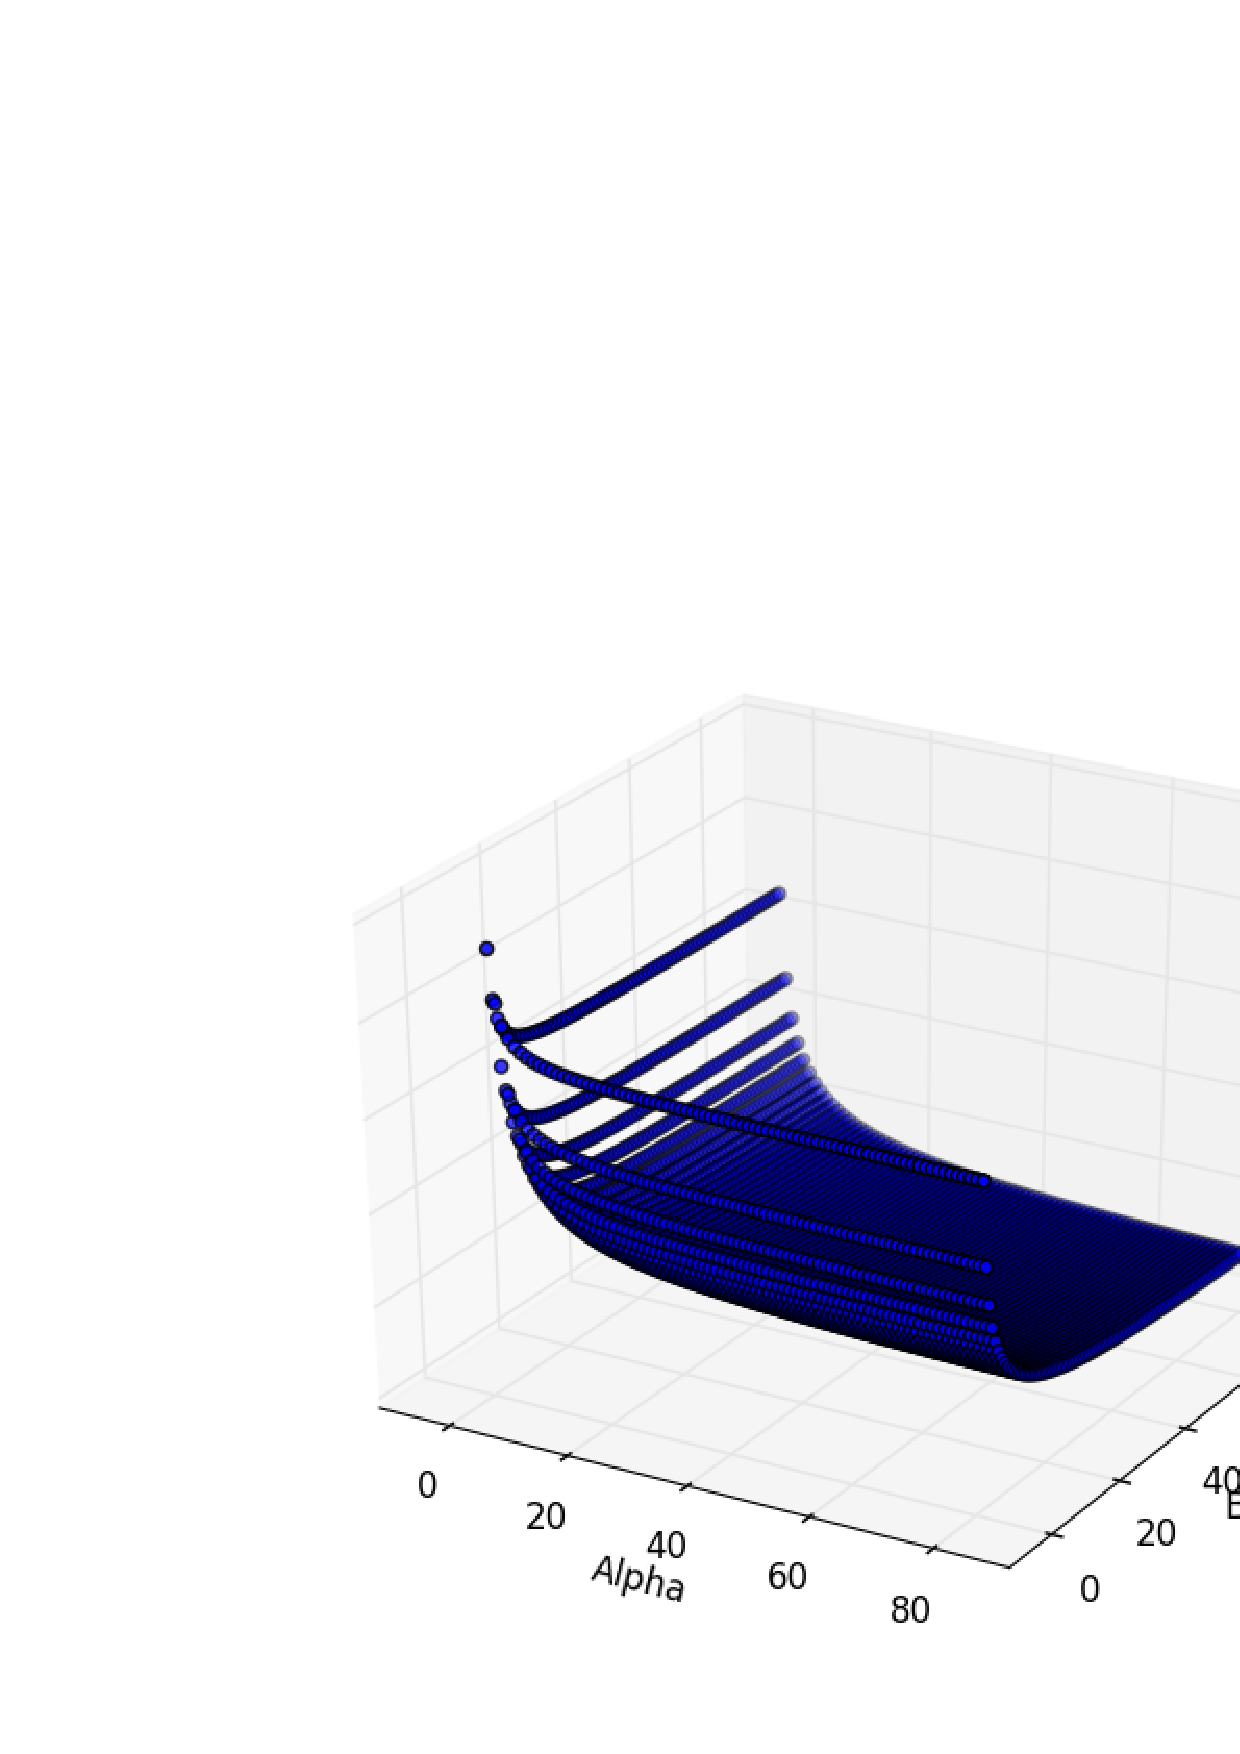
\includegraphics[width=0.48\textwidth]{sensitivity}
\caption{Hellinger distance study}
\label{fig_sensitivity}
\end{figure}
In this part, we firstly study the local sensitivity of Hellinger distance of different $\betad$ distributions as in Fig. \ref{fig_sensitivity}, in order to have a better understanding of the relationships between accuracy and next two aspects.


As in Fig. \ref{fig_sensitivity}, the local sensitivity of Hellinger distance will decrease when $\betad$ distribution's two parameters get closer (i.e. more uniform) and larger. In the same time, our smooth sensitivity will also decrease based on the Def. \ref{def_smoo}. From accuracy bound in Sec. \ref{subsec_accuracy_smoo}, the accuracy will be improved when sensitivity go larger. In consequence, when we increase the prior distribution, the smooth sensitivity in our exponential mechanism will decrease, which means our accuracy will be improved. However, the sensitivity of $l_1$ norm in Laplace mechanism is fixed regardless the prior distribution. We will study this trade-off in Sec. \ref{subsubsec_vs_prior}.

\subsubsection{Accuracy Analysis wrt. data variance}

Similar as above, when the data variance is small (i.e. the data are uniform), the parameters of posterior distribution will get more uniform (i.e. closer). Based on Fig. \ref{fig_sensitivity}, the Hellinger distance's sensitivity will get smaller when parameter get closer. As a result, the accuracy will be improved in the same time. We will study this trade-off in Sec. \ref{subsubsec_vs_variance}


\begin{figure}[ht]
\centering
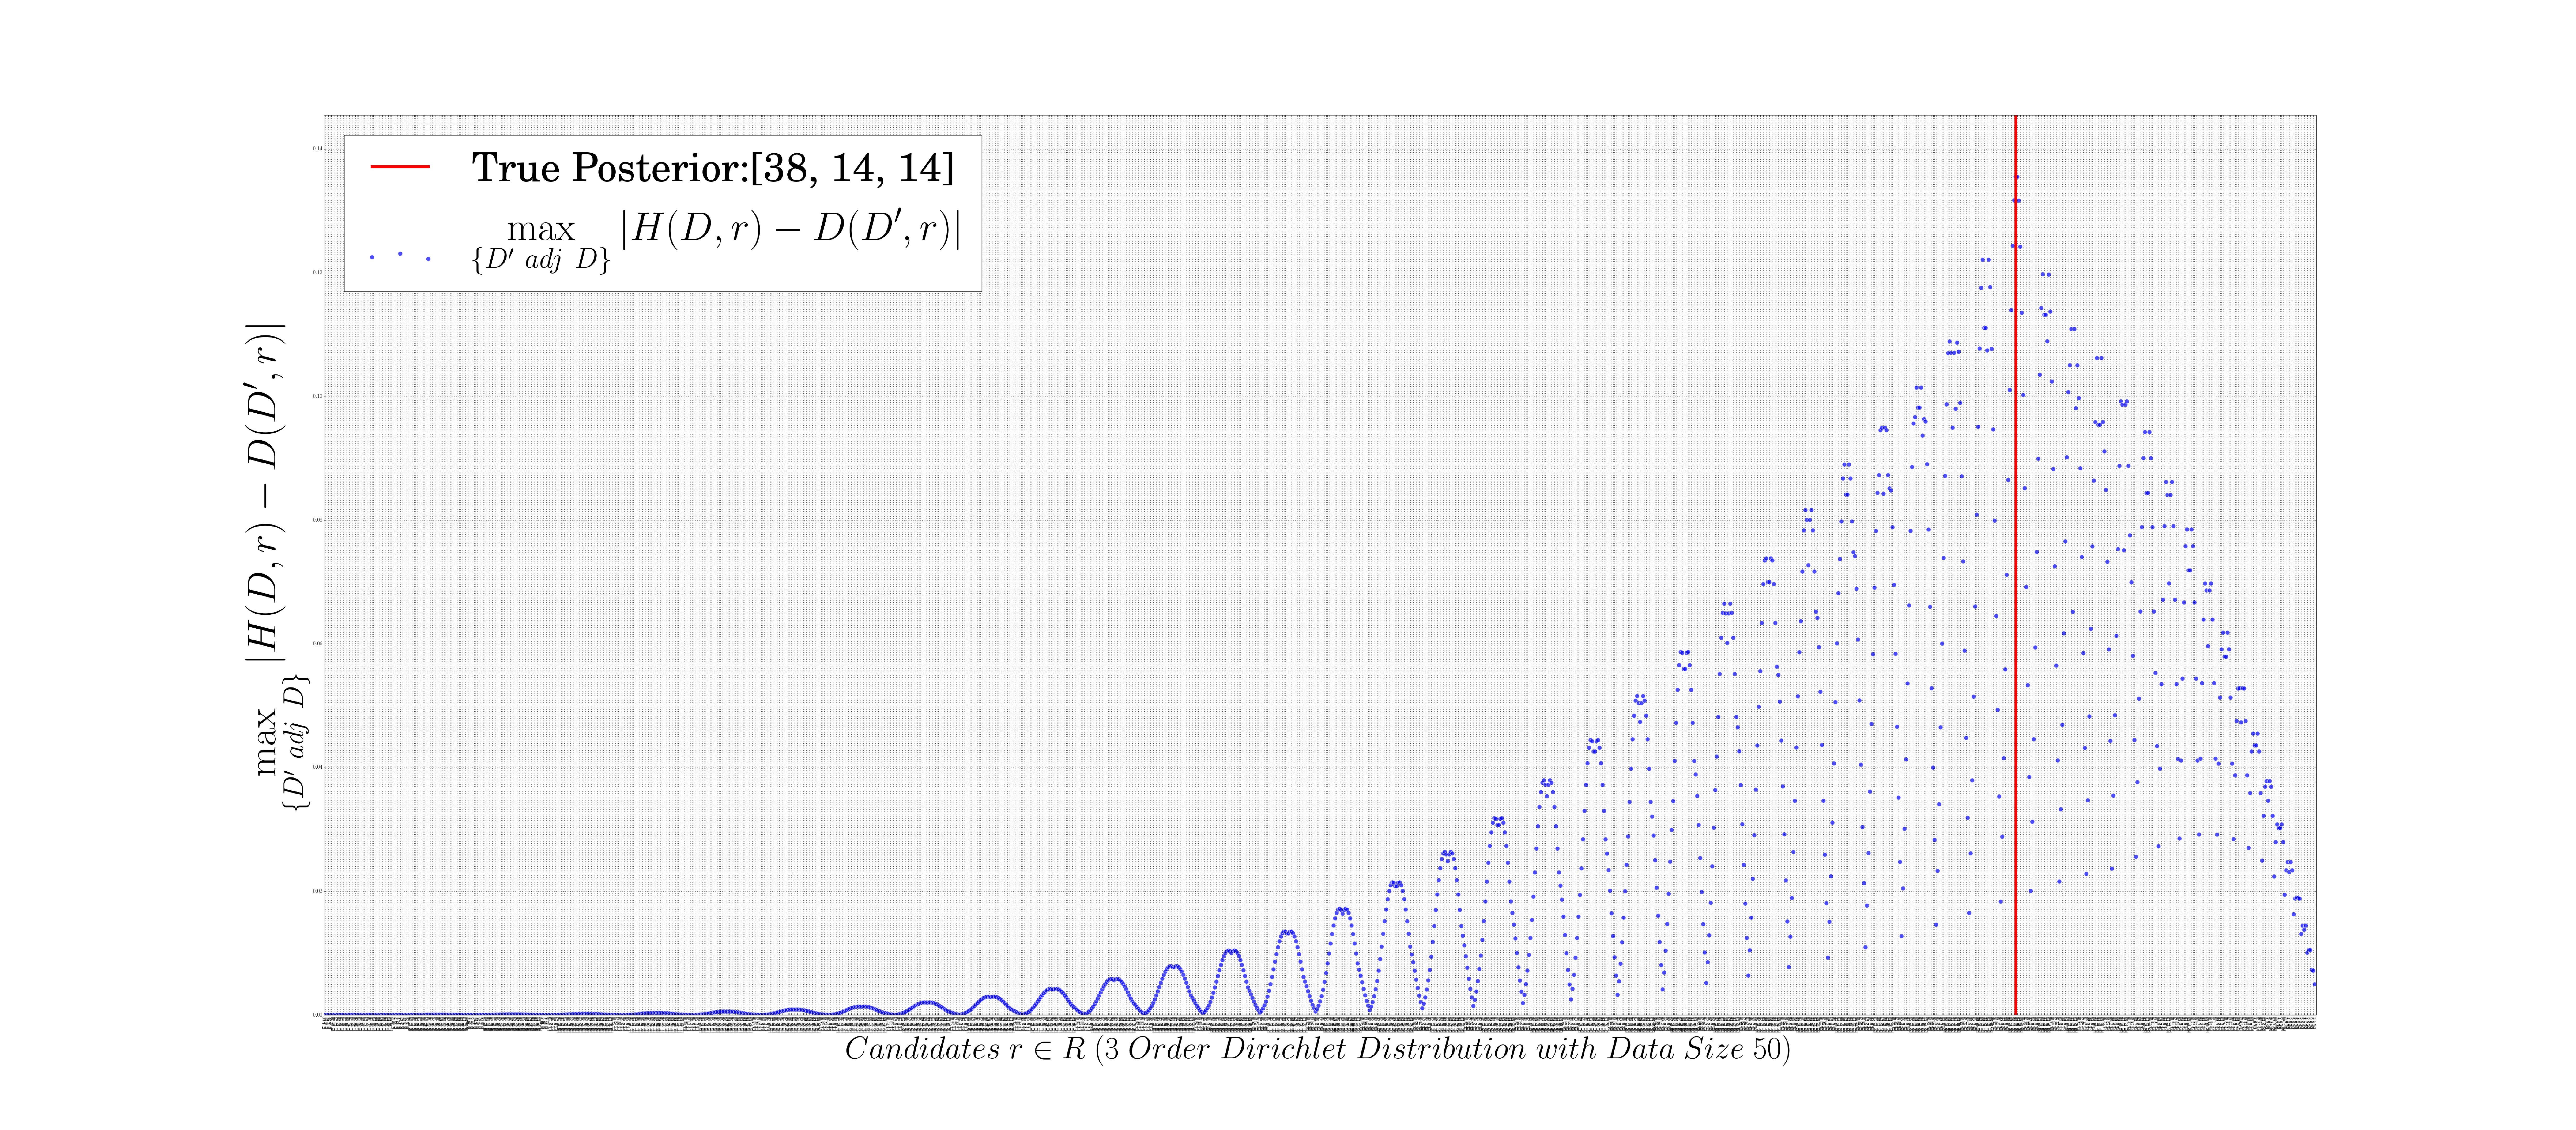
\includegraphics[width=0.48\textwidth]{efficiency}
\label{fig_efficiency}
\caption{Experimental Results for Finding the Local Sensitivity Efficiently}
\end{figure}


\section{Experimental Evaluations}
\label{sec_experiment}

\subsection{Computation Efficiency}
\label{subsec_effi}
The formula for computing the local sensitivity presented in Sec. \ref{subsec_emls}:$\max\limits_{\{|x,y'| \leq 1; y'\in \mathcal{X}^n\}}\max\limits_{\{r\in R\}} \{\hlg(\bysinfer(x), r) - \hlg(\bysinfer(y'), r)|\}$ can be reduced to $\max\limits_{\{|x,y'| \leq 1;y'\in \mathcal{X}^n\}}\hlg(\bysinfer(x), \bysinfer(y'))|$ by applying the distance triangle property. i.e., the maximum value over $\max\limits_{r \in R}$ always happen when $r = \bysinfer(x)$ itself, where $\Delta_{l}u(x) = \max\limits_{\{|x,y'| \leq 1;y'\in \mathcal{X}^n\}} \{\hlg(\bysinfer(x), \bysinfer(x)) - \hlg(\bysinfer(y'), \bysinfer(x))|\} = \max\limits_{\{|x,y'| \leq 1;y'\in \mathcal{X}^n\}} \{\hlg(\bysinfer(y'), \bysinfer(x))|\}$. We also have some experiments for validating our proposal as in Fig. \ref{fig_efficiency}, where we calculate the $\max\limits_{\{|x,y'| \leq 1;y'\in \mathcal{X}^n\}}$ value for every candidate $r \in R$. It is shown that maximum value taken when  $r = \bysinfer(x)$.


\subsection{Accuracy Trade-off Evaluation wrt. Different Variables}
\label{subsec_vs_variables}
In this section, we evaluate the accuracy of the mechanisms defined in
Section (\ref{sec_smoo}) w.r.t. four variables, including data size, dimensions,
data variance, prior distribution, and some combinations thereof.
Every plot is an average over 1000 runs. In all the experiments we set
$\epsilon = 0.8$, and $\delta = 10^{-8}$.

\noindent In the following some of the plots show
mean error as a function of the datasize while one
is a whiskers-plot where the y-axis shows the average
accuracy (or equivalently, the error) of the mechanisms, and the x-axis, instead shows
different balanced priors used. The boxes extend from the lower to the upper quartile values
of the data, with a line at the median. A notch on the box around the
median is also drawn to give a rough guide to the significance of
difference of medians; The whiskers extend from the box to show the
range of the data. A blue box in the plots represents our newly
designed exponential mechanism's behavior-- where the sensitivity is calibrated
w.r.t Hellinger distance-- while the yellow box next to
it represents the performance of a variation of the basic Laplace
mechanism presented in Section (\ref{sec:base}) with the same
settings: that is $\epsilon, \delta$, data, prior. The variation
considered performs a postprocessing on the released parameters so
that they are consistent. For instance when the sum of the noised
parameters is greater than $n$ we will truncate them so that they sum
up to $n$.

\paragraph{Increasing data size with balanced datasets}
\label{subsubsec_vs_datasize}

\begin{figure}[H]
\begin{center}
\centering
  \subfigure[Data set size from $300$ to $800$ ]{
    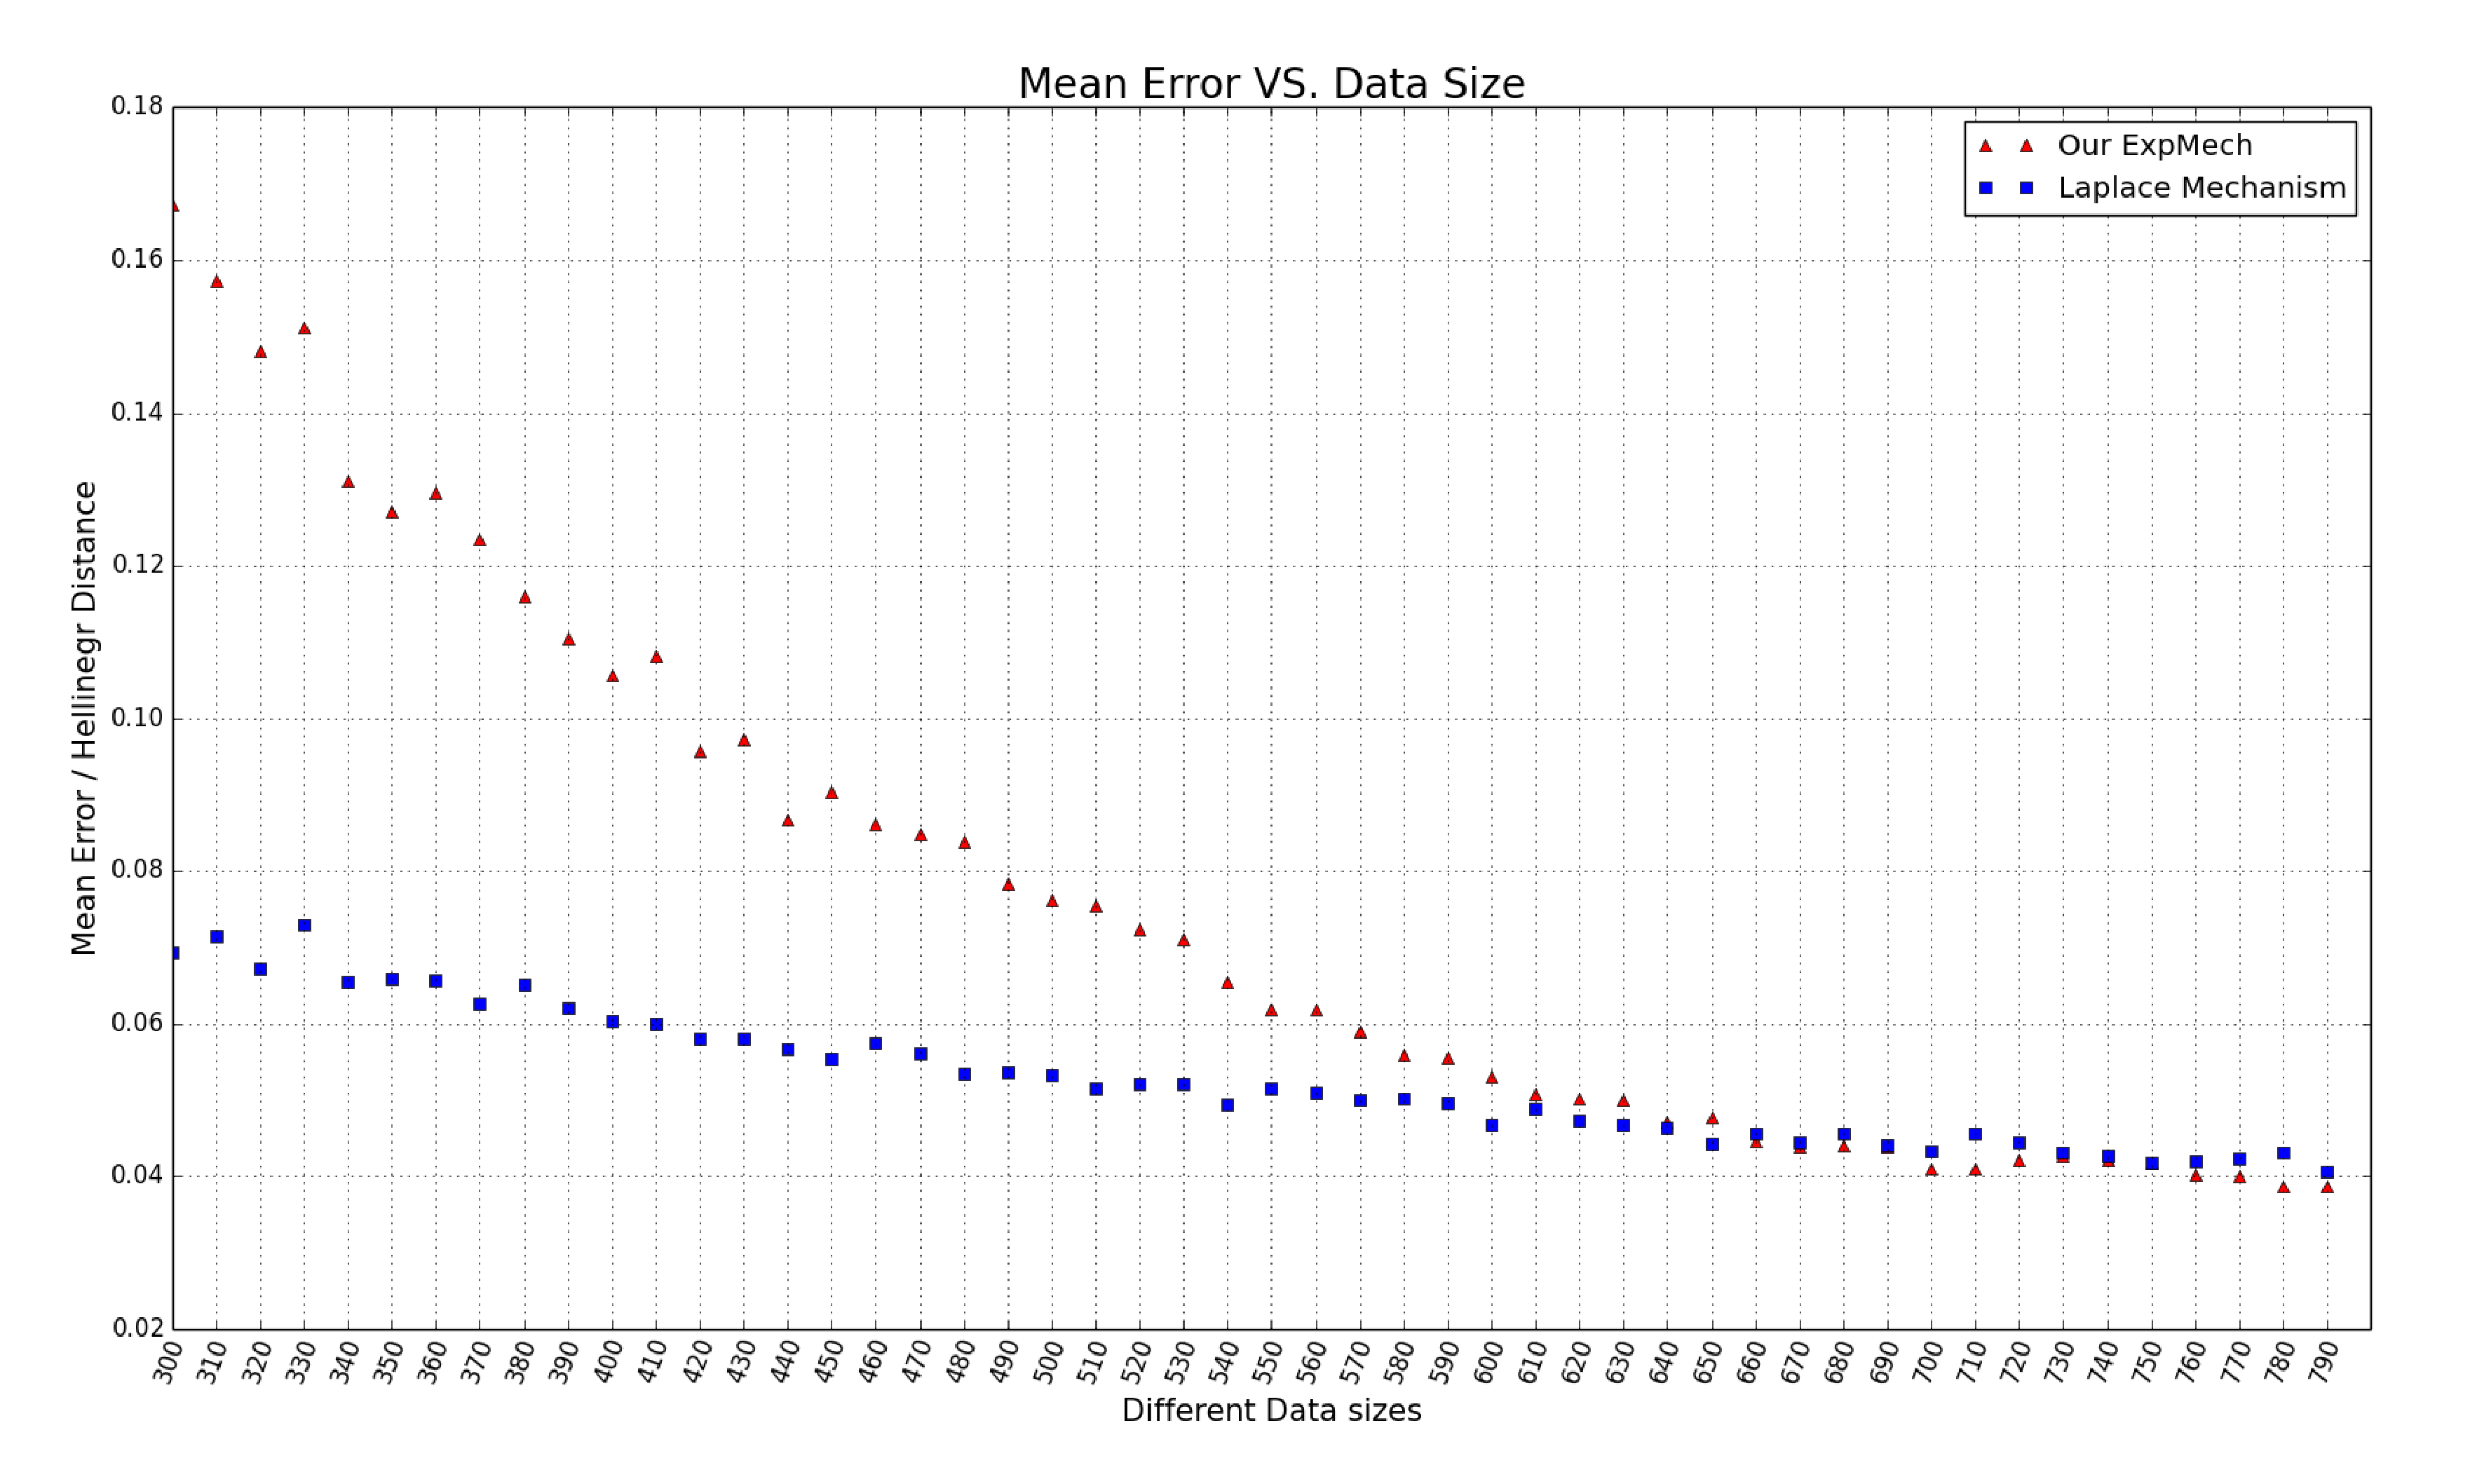
\includegraphics[width=0.45\textwidth]{accuracy_vs_datasize_800.eps}
    \label{subsubsec_vs_datasize1a}
  }
  \subfigure[Data set size from $14000$ to $20000$]{
    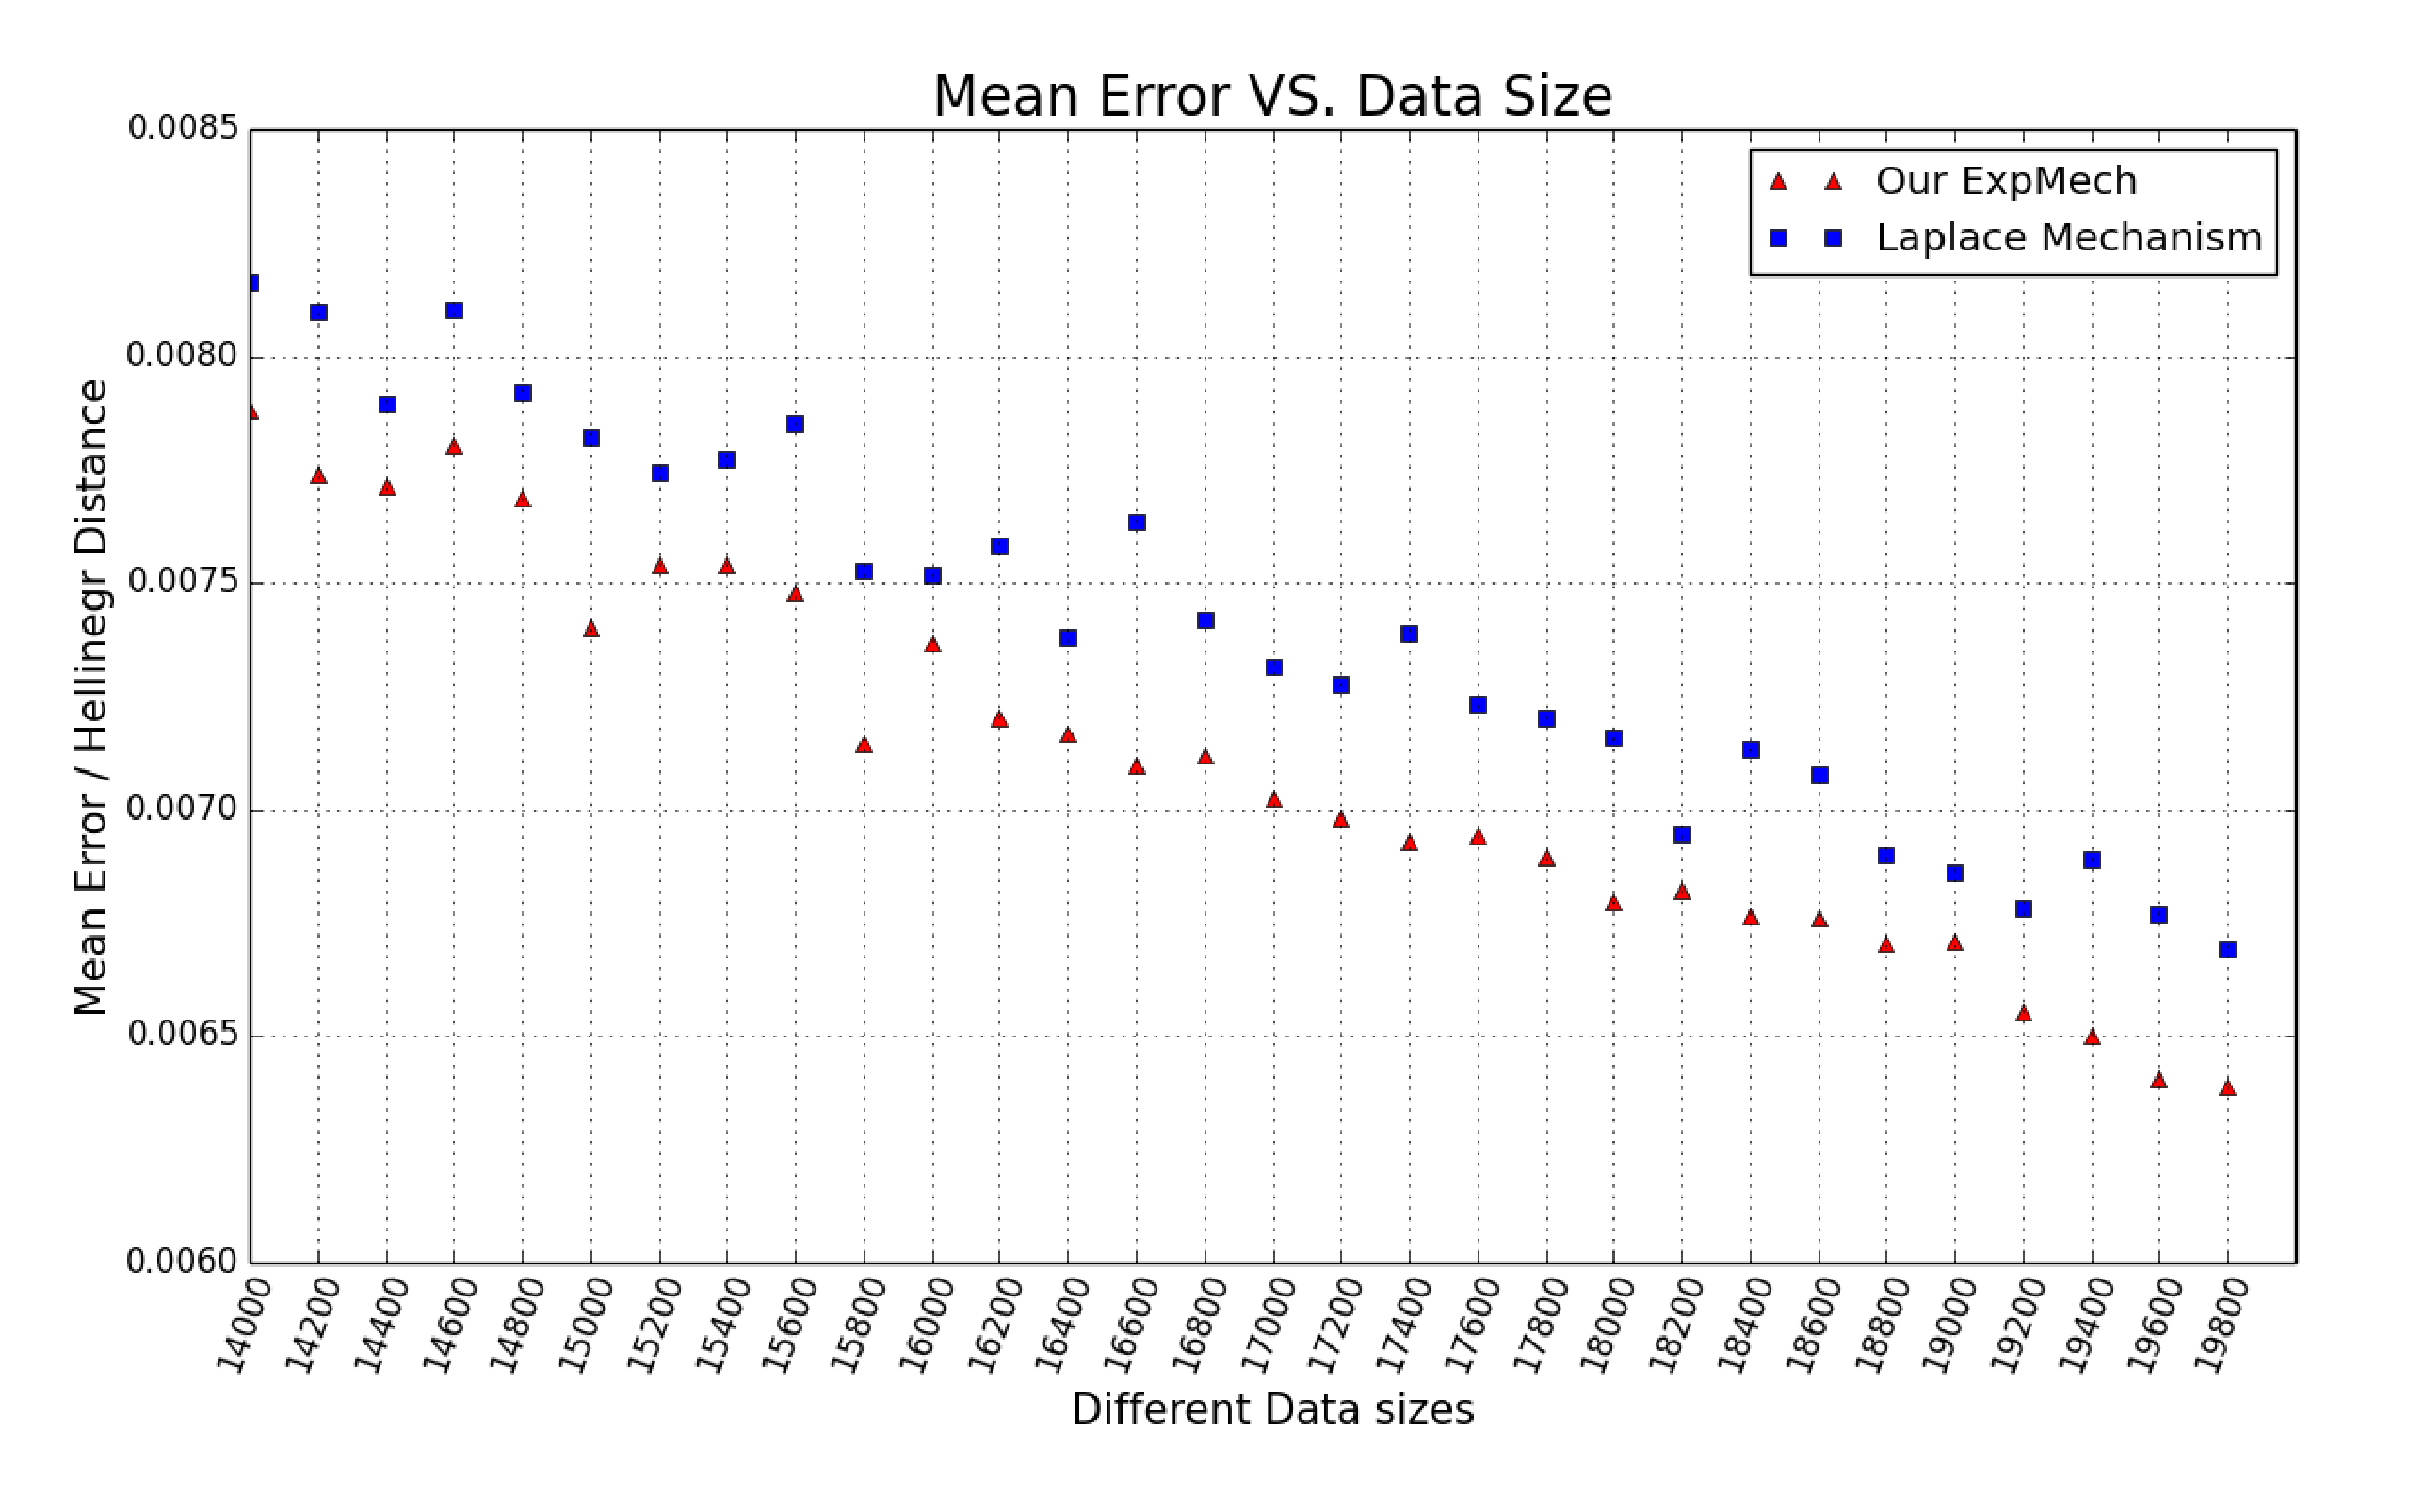
\includegraphics[width=0.45\textwidth]{accuracy_vs_datasize_20000.eps}
  \label{subsubsec_vs_datasize1b}} 
\caption{Increasing data size with fixed prior $\betad(1,1)$. Unbalanced datasets of mean $(0.1,0.9)$ and parameters $\epsilon = 0.8$ and $\delta = 10^{-8}$}
\label{fig_vs_datasize}
\end{center}
\end{figure}

\begin{figure}[ht]
\begin{center}
\centering
  % \subfigure[Data set size from $300$ to $800$ ]{
  %   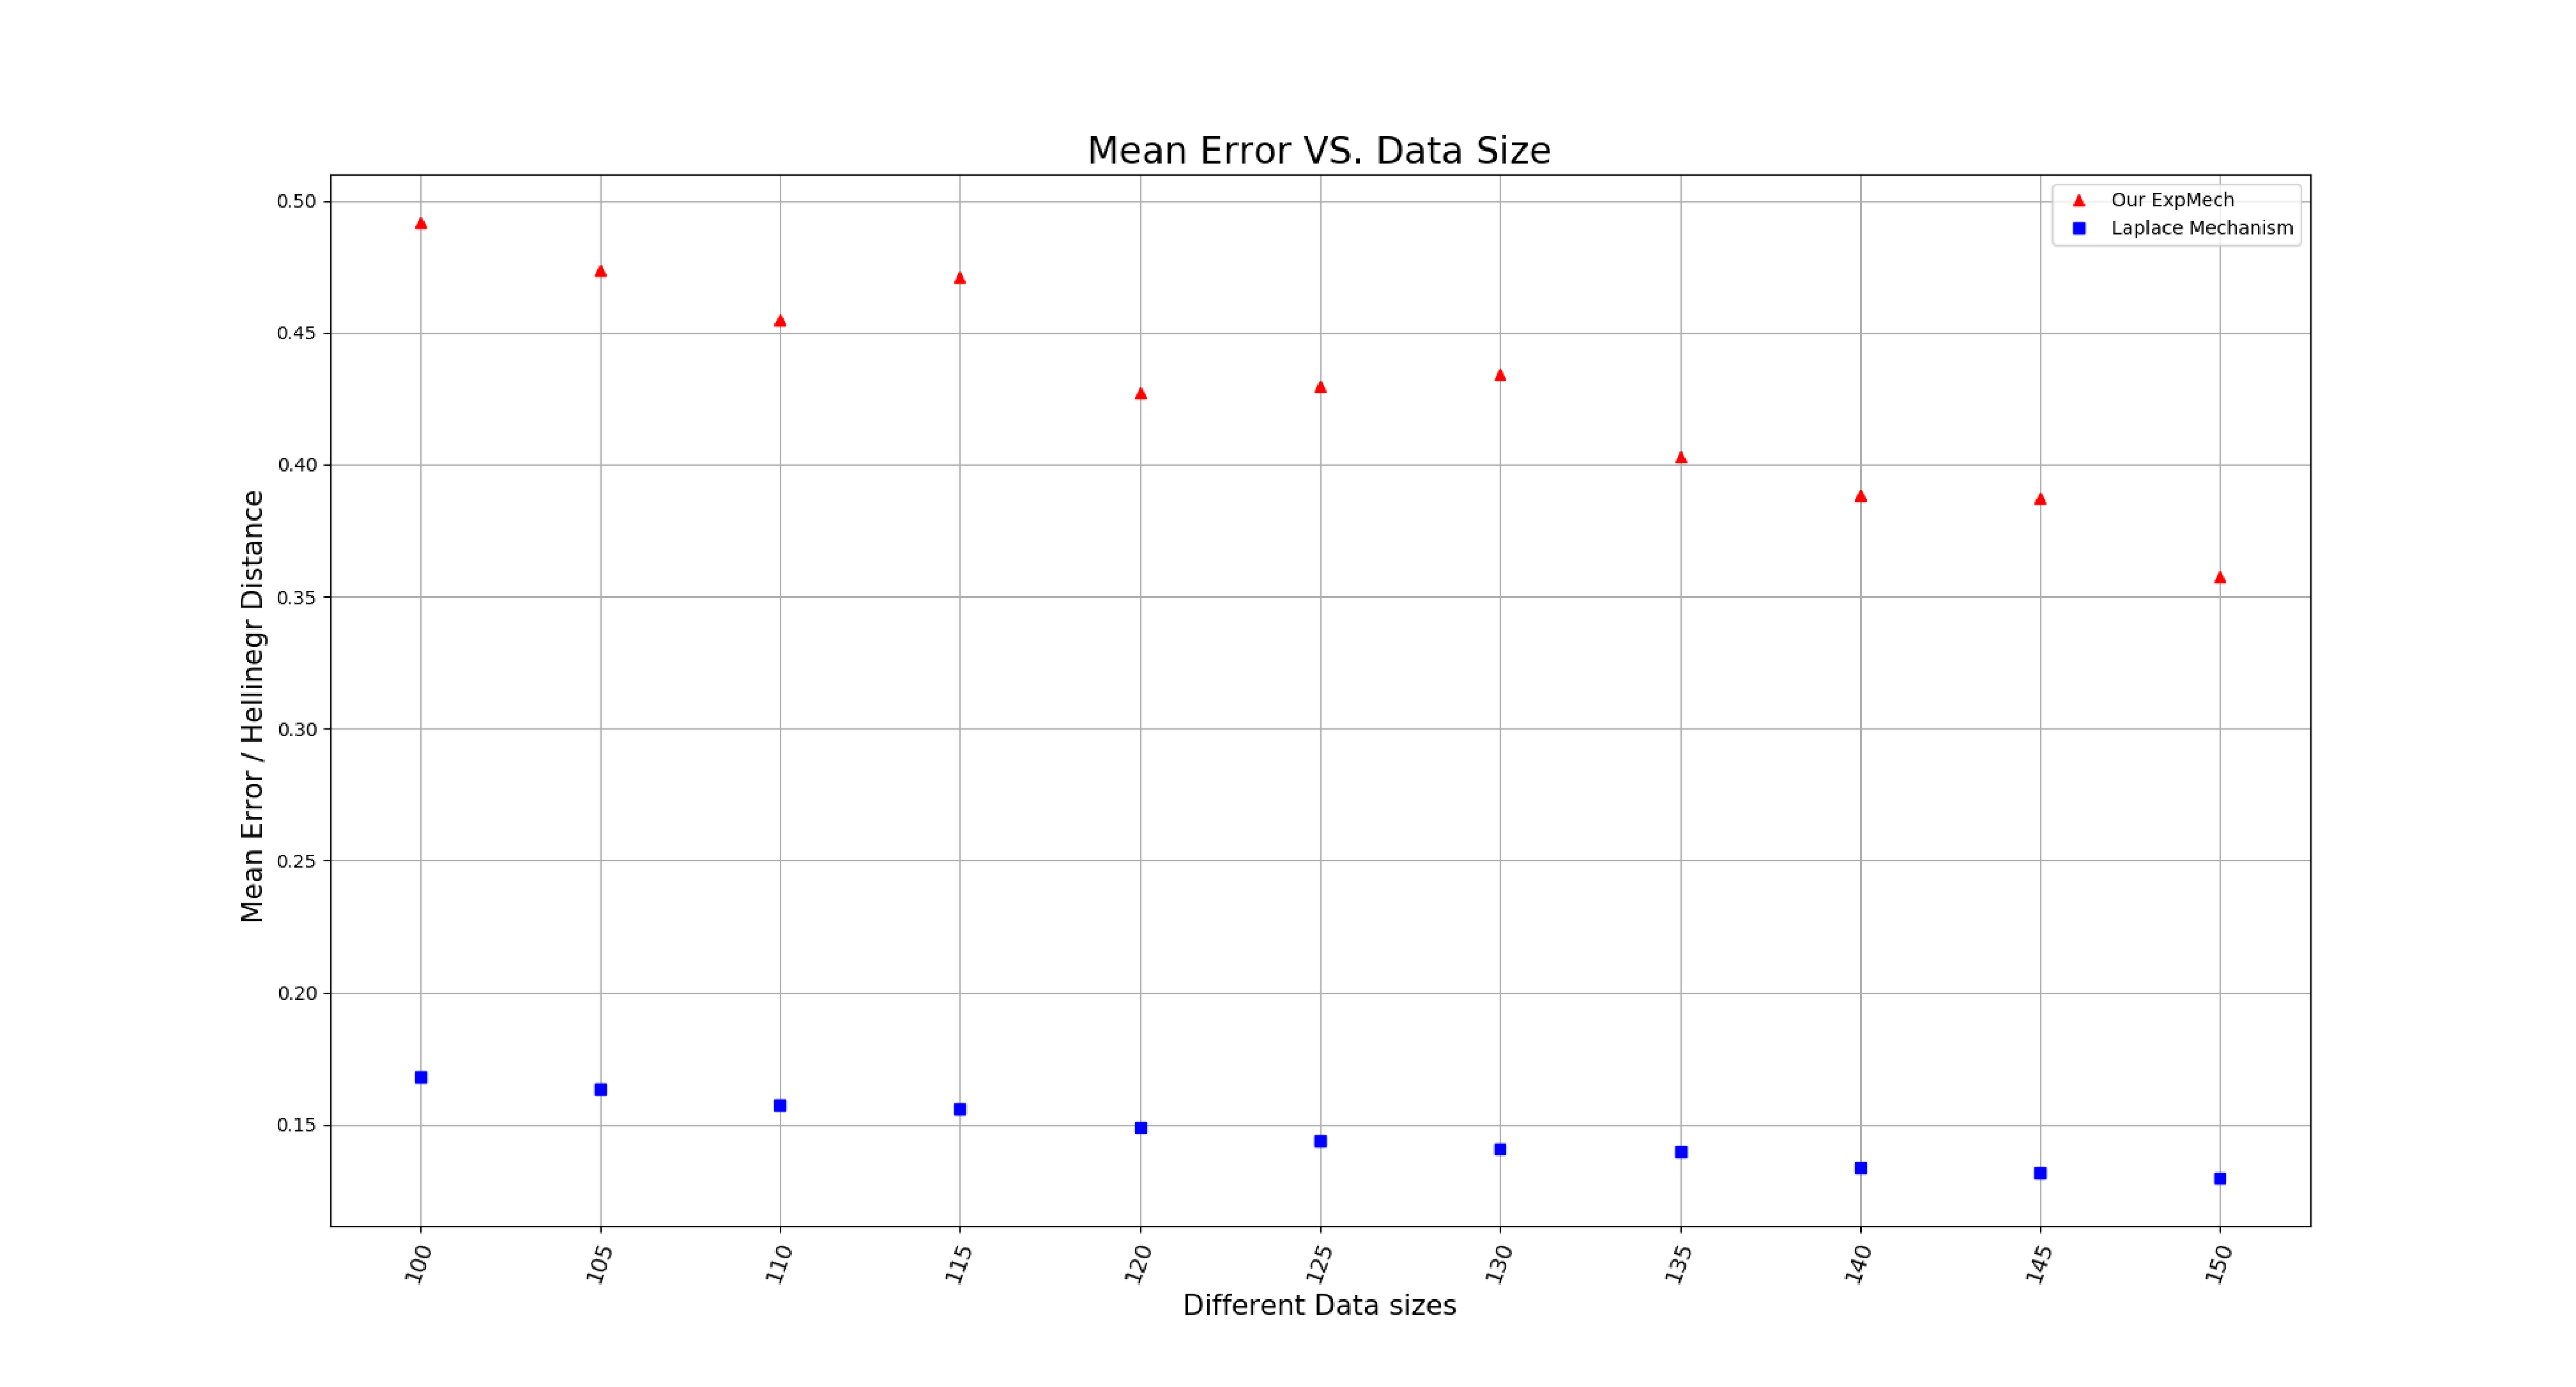
\includegraphics[width=0.45\textwidth]{accuracy_vs_datasize_300_dirichlet.eps}
  %   \label{subsubsec_vs_datasize1adir}
  % }
  \subfigure[Data set size from $14000$ to $20000$]{
     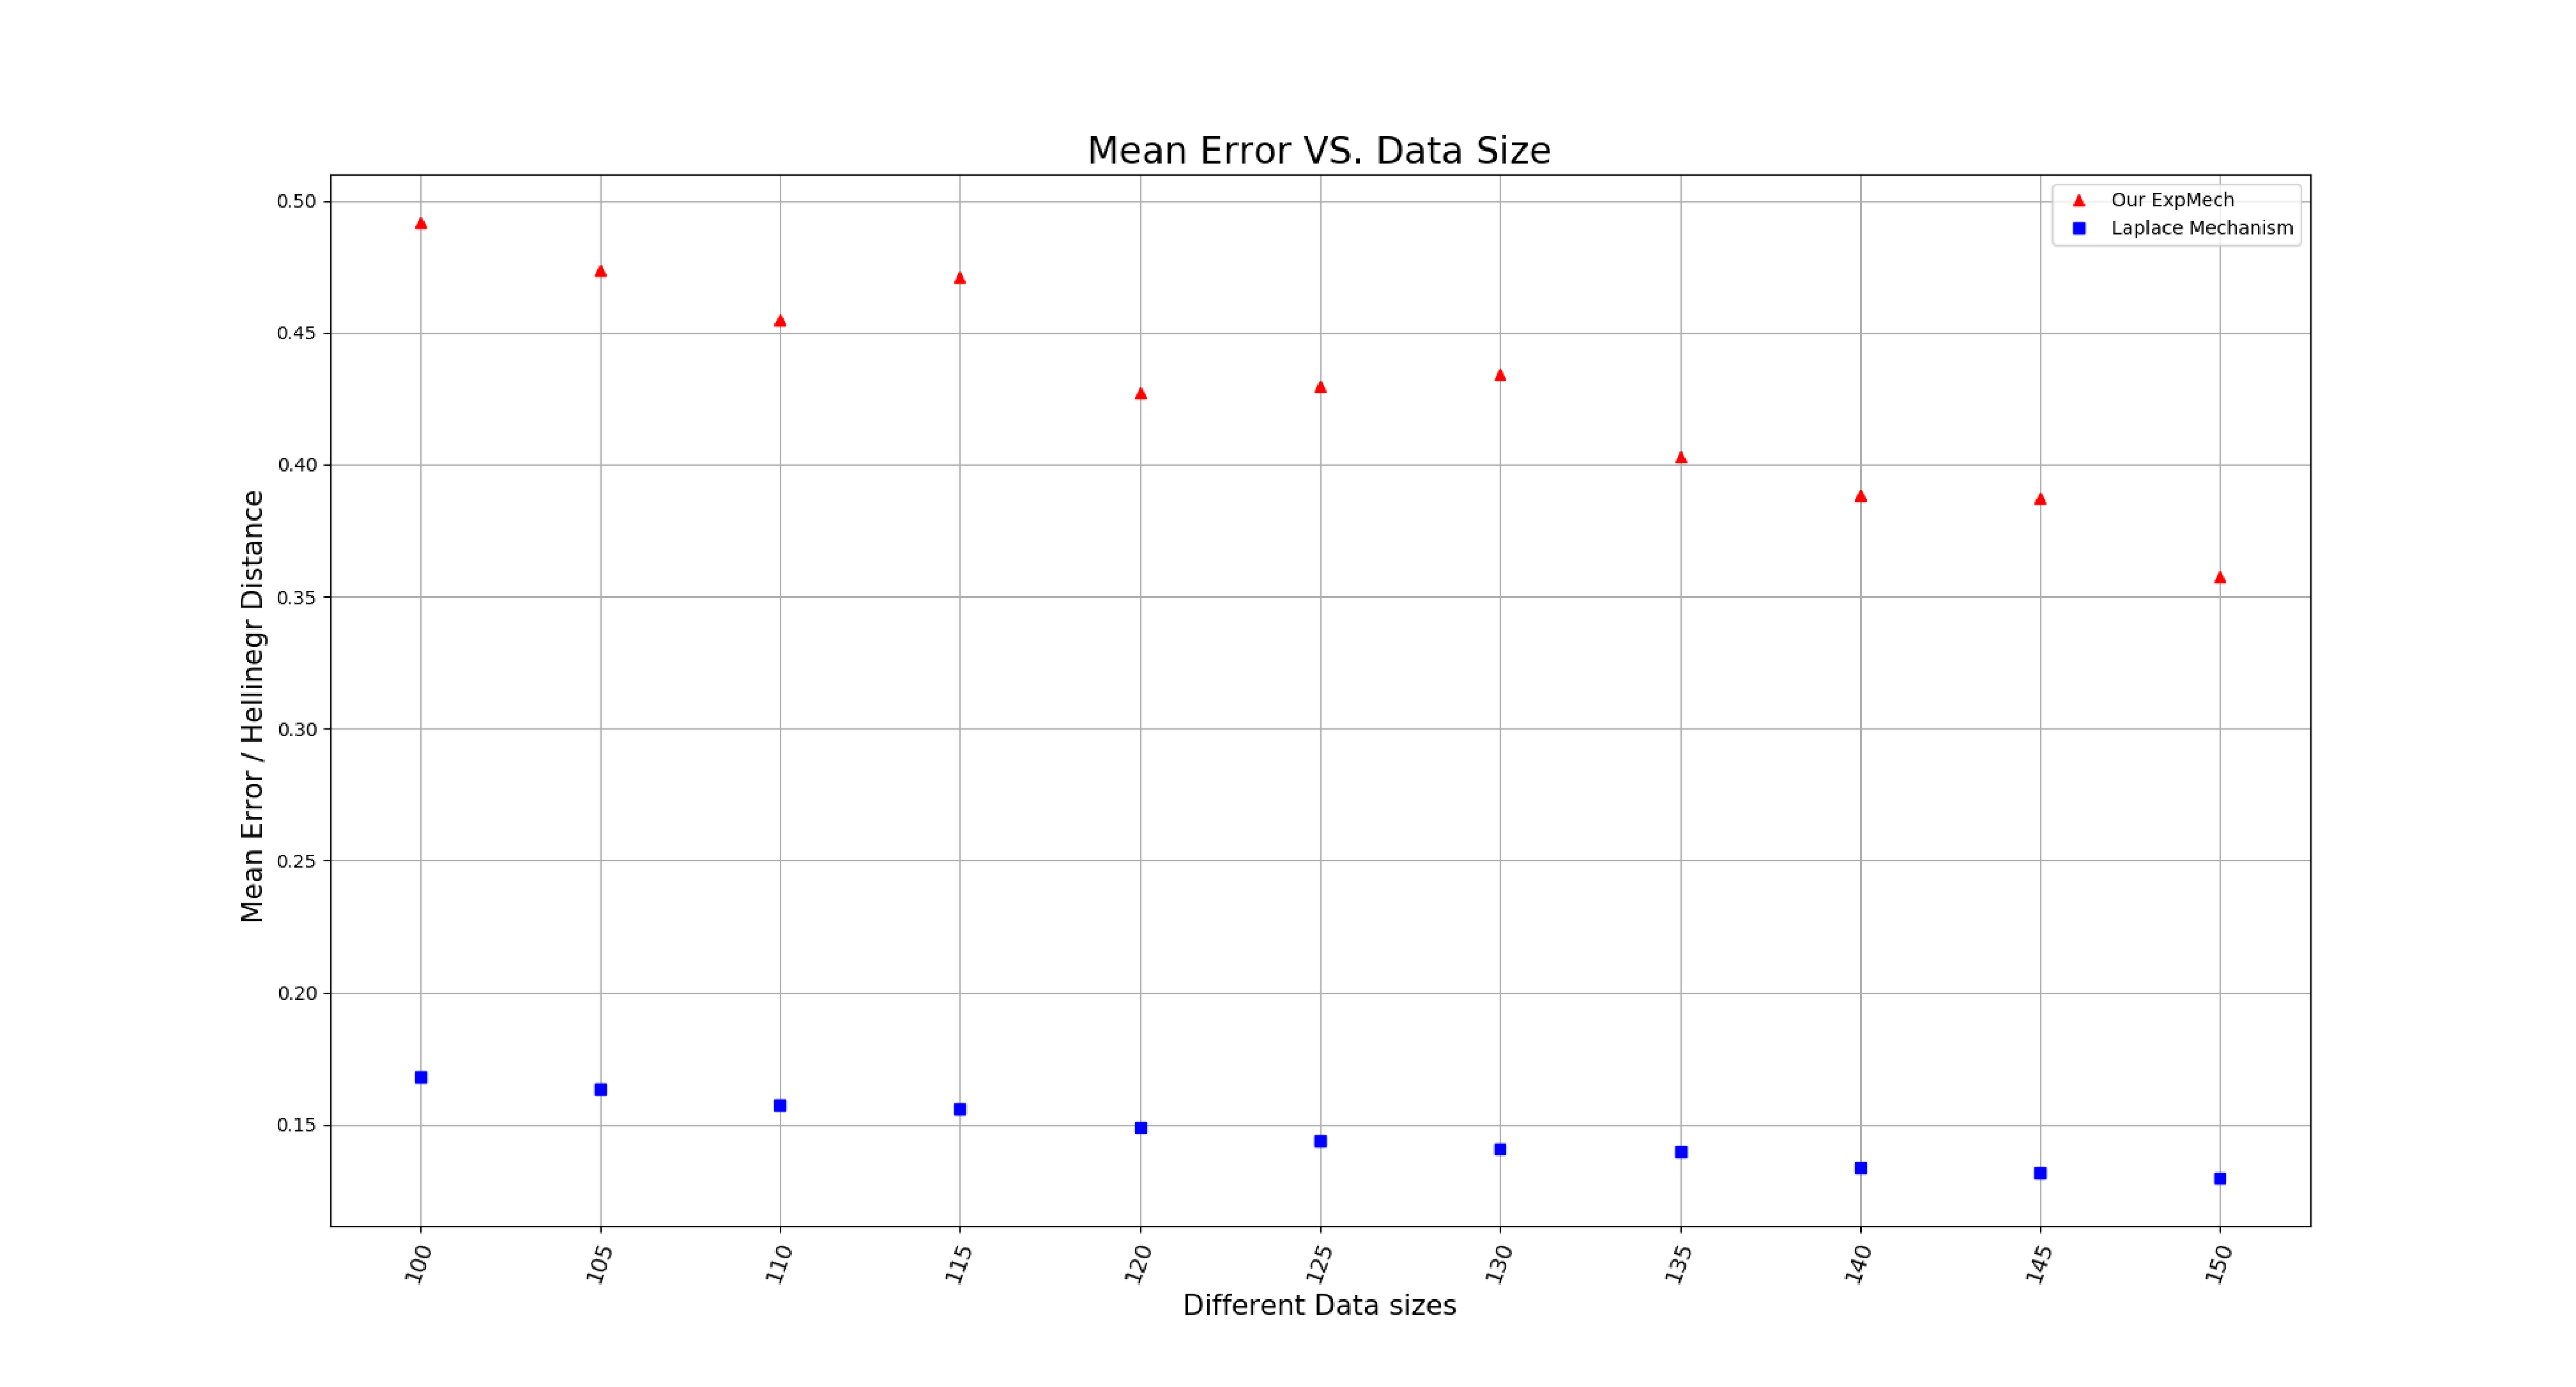
\includegraphics[width=0.45\textwidth]{accuracy_vs_datasize_1k_dirichlet.eps}   
  \label{subsubsec_vs_datasize1bdir}
  } 
\caption{Increasing data size with fixed $\dirichlet(1,1,1)$ prior distribution, Unbalanced datasets of mean $(0.2,0.3, 0.5)$ and parameters $\epsilon = 0.8$ and $\delta = 10^{-8}$}
\label{fig_vs_datasize_dir}
\end{center}
\end{figure}

In Figures \ref{fig_vs_datasize} and \ref{fig_vs_datasize_dir} we consider \emph{unbalanced} datasets
of observations. This means that in the Beta-Binomial setting (Figure \ref{subsubsec_vs_datasize1a},
and \ref{subsubsec_vs_datasize1b}) the datasets will consist of 10\% 1s and the rest 0s, while for the
Dirichelet-Multinomial (Figure  \ref{subsubsec_vs_datasize1adir} and \ref{subsubsec_vs_datasize1bdir})
the data will be split in the $k=3$ bins with perecentages of: 20\%, 30\% and 50\%.
The results show that when the data size
increases, the average errors of
$\hexpmech$, $\hexpmechd$, and Laplace decrease. For small datasets,
i.e with size less 650 in the case of Beta-Binomial systems,
the Laplace mechanisms outperforms the exponential mechanisms,
but for bigger data sets, that is, bigger than 650, or as in Figure \ref{subsubsec_vs_datasize1b} where
we considered data sets of the order of 15 thousands elements,
the exponential mechanisms outperforms the Laplace mechanism.
Similar experimental tendencies were obtained for the Dirichlet-Multinomial system ( (Figure  \ref{subsubsec_vs_datasize1adir} and \ref{subsubsec_vs_datasize1bdir})),
but we were not able to perform experiments with higher dimensions (4 or more) or, big datasets, e.g. $10^4$ elements, due to
too high run time of the algorithm.




\paragraph{Fixed dataset varying balanced priors}
\label{subsubsec_vs_prior}
In Figure \ref{fig_vs_prior}, we fix the dataset to be $\langle 5,5,5\rangle$.
We also considered balanced priors with increasing values in their dimensions.
The plot shows that in the beginning the Laplace mechanism performs better but
it is outperformed after a while.
\begin{figure}[H]
\centering
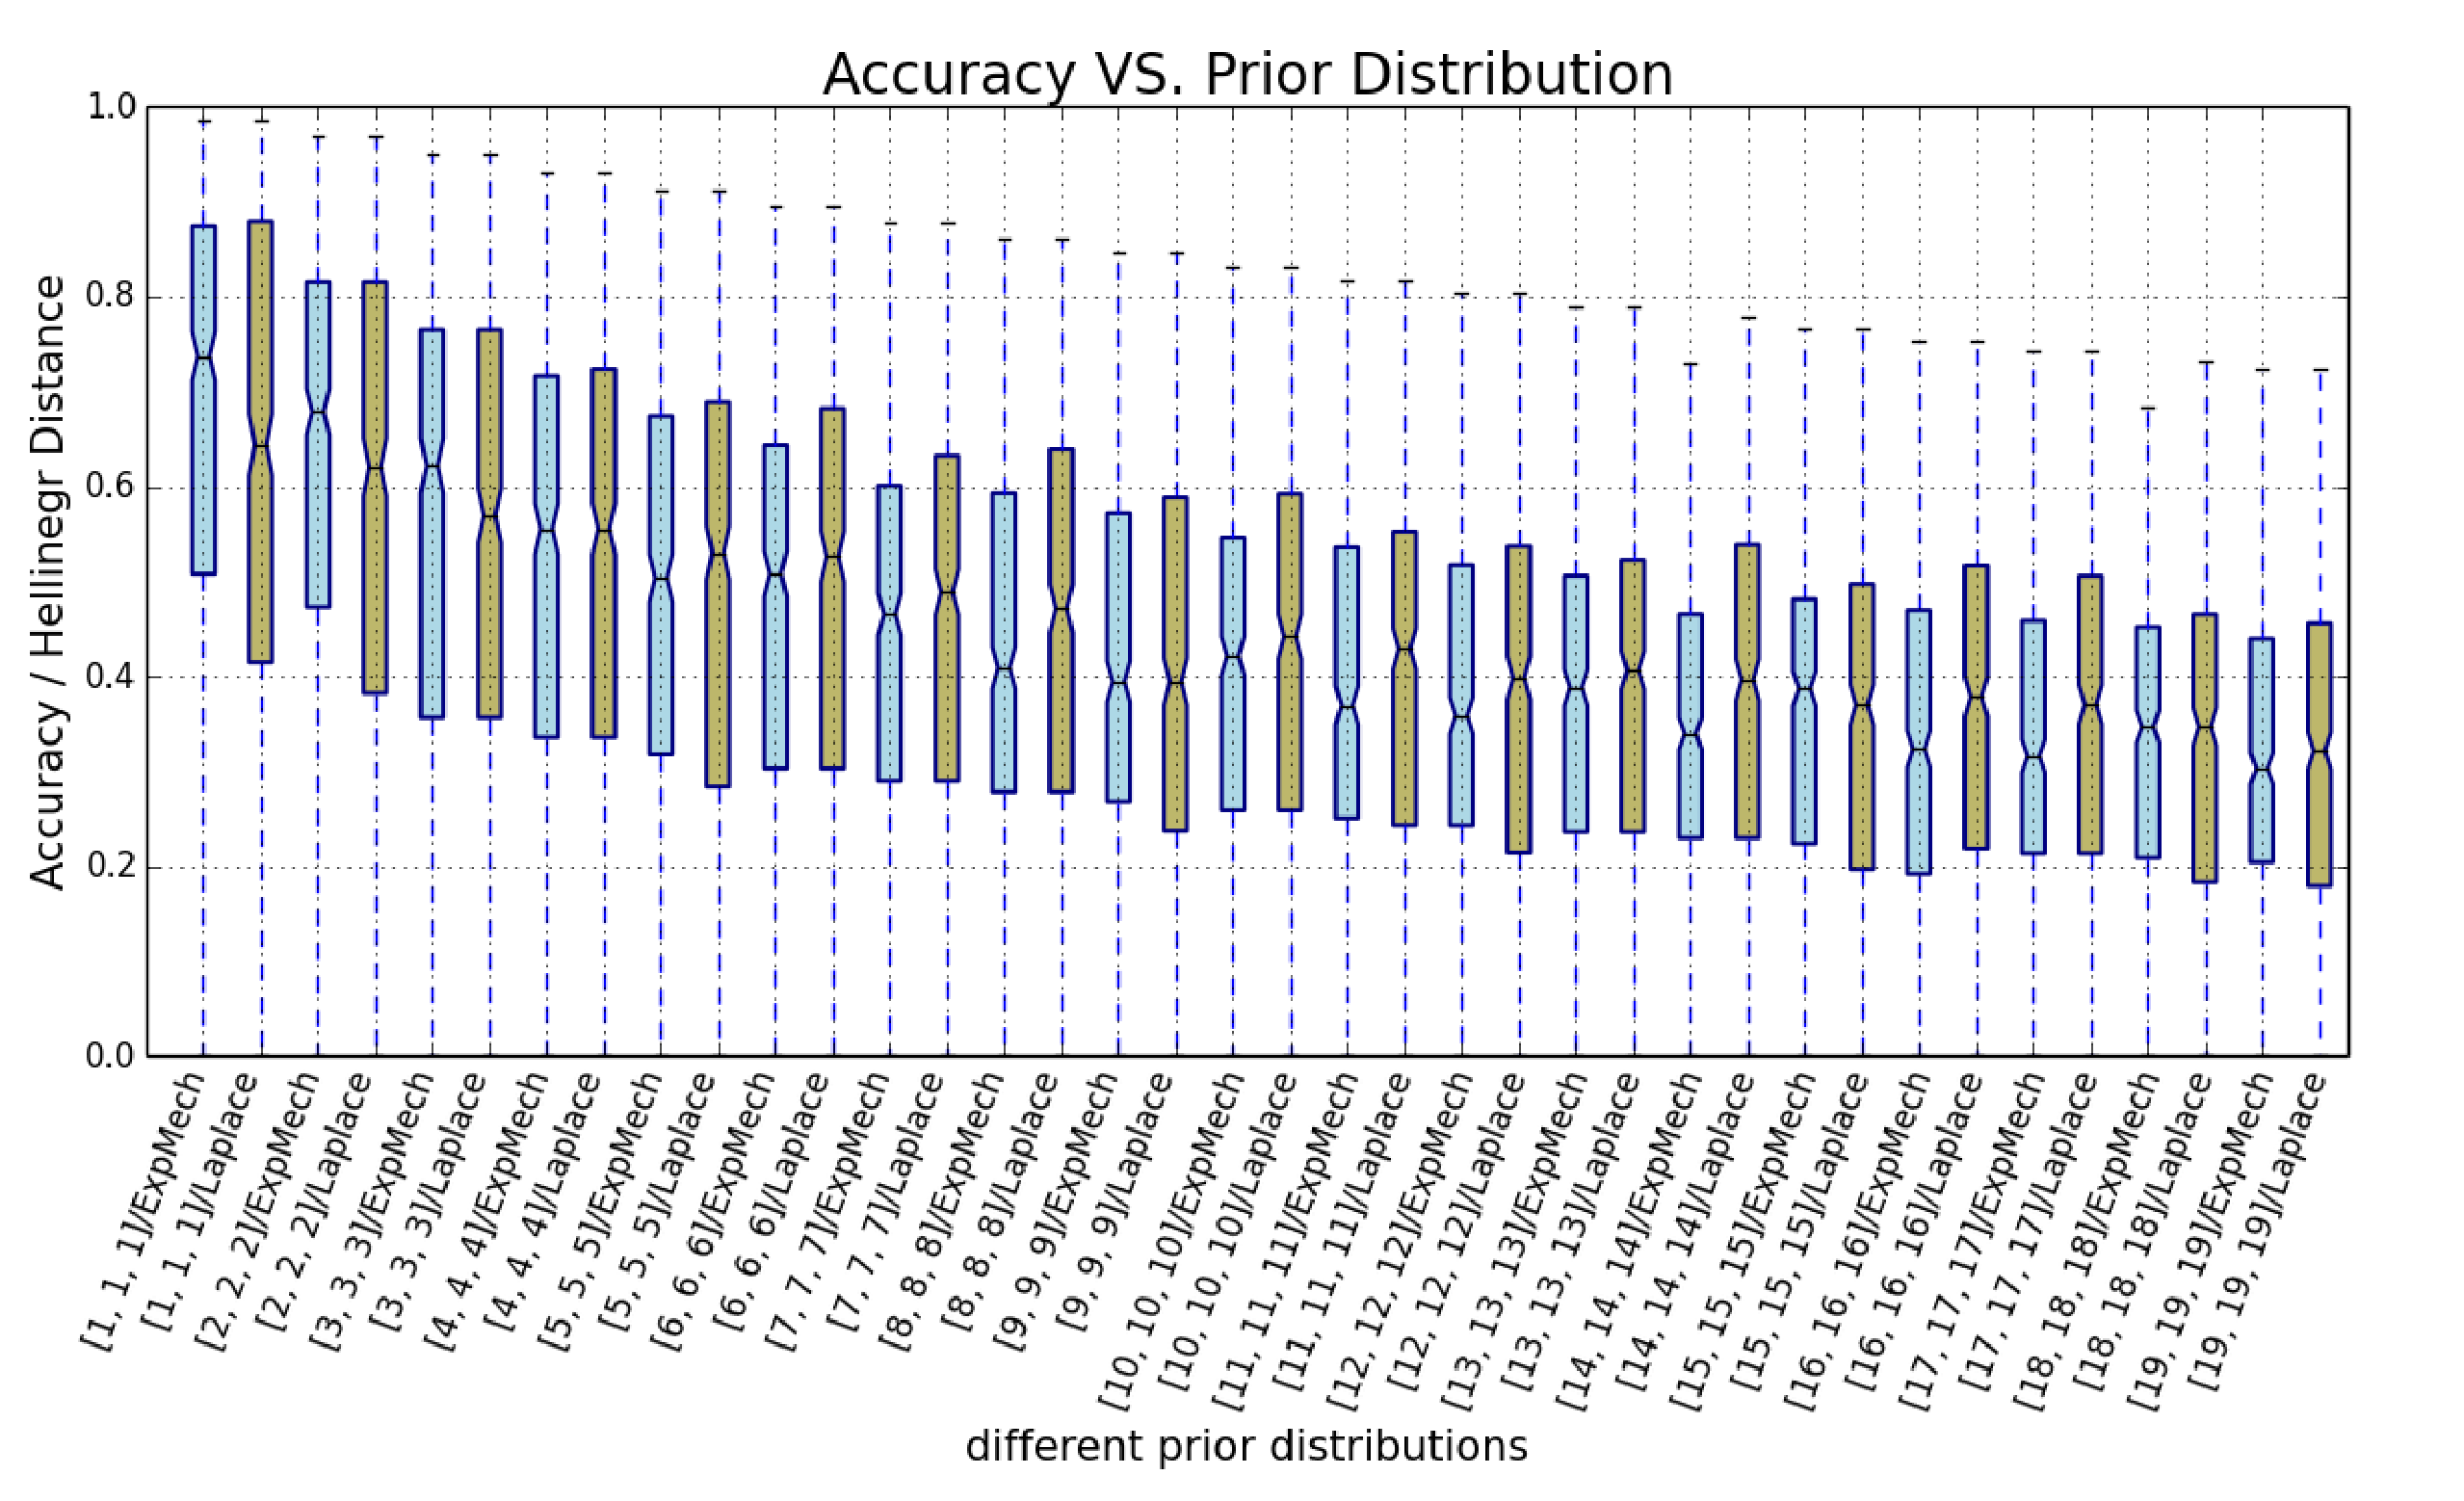
\includegraphics[width=0.45\textwidth]{accuracy_vs_prior_5_5_5.eps}
\caption{Observed data set is: $(5,5,5)$, varying balanced priors}
\label{fig_vs_prior}
\end{figure}

\subsection{Experiment Evaluations on Privacy}
\label{subsec_experiment_privacy}
In order to see our privacy behavior, we study the accurate epsilon under concrete cases in this section. The $(\epsilon, \delta)$ - differential privacy we proved in Sec. \ref{sec_smoo} is just an upper bound, we concrete $\epsilon$ should be smaller than upper bound in our exponential mechanism. We calculate the concrete privacy value in following ways wrt. the data size, and obtain plots in Fig. \ref{fig_privacy}.

\begin{figure*}
\begin{center}
\centering
  \subfigure[data size range from 90 to 180]{
    \includegraphics[width=0.45\textwidth]{global_epsilon_20_20.eps}}
  \subfigure[data size range from 90 to 180]{
    \includegraphics[width=0.45\textwidth]{global_epsilon_20_20(2).eps}} 
\caption{Concrete privacy calculation under settings that: prior distribution:$[1,1]$, $\epsilon = 0.8$, $\delta = 0.0005$ and observed data are uniformly distributed}
\label{fig_privacy}
\end{center}
\end{figure*}

$\epsilon = 0.8$ is a privacy upper bound, we can observe that the concrete $\epsilon$ values are smaller than the upper bound. That is to say, we achieved a higher privacy level than expected. In next step, we are going to improve the accuracy using this property.


\bibliographystyle{ACM-Reference-Format}
\bibliography{bayesian.bib}

\end{document}

